% Template for Elsevier CRC journal article
% version 1.2 dated 09 May 2011

% This file (c) 2009-2011 Elsevier Ltd.  Modifications may be freely made,
% provided the edited file is saved under a different name

% This file contains modifications for Procedia Computer Science

% Changes since version 1.1
% - added "procedia" option compliant with ecrc.sty version 1.2a
%   (makes the layout approximately the same as the Word CRC template)
% - added example for generating copyright line in abstract

%-----------------------------------------------------------------------------------

%% This template uses the elsarticle.cls document class and the extension package ecrc.sty
%% For full documentation on usage of elsarticle.cls, consult the documentation "elsdoc.pdf"
%% Further resources available at http://www.elsevier.com/latex

%-----------------------------------------------------------------------------------

%%%%%%%%%%%%%%%%%%%%%%%%%%%%%%%%%%%%%%%%%%%%%%%%%%%%%%%%%%%%%%
%%%%%%%%%%%%%%%%%%%%%%%%%%%%%%%%%%%%%%%%%%%%%%%%%%%%%%%%%%%%%%
%%                                                          %%
%% Important note on usage                                  %%
%% -----------------------                                  %%
%% This file should normally be compiled with PDFLaTeX      %%
%% Using standard LaTeX should work but may produce clashes %%
%%                                                          %%
%%%%%%%%%%%%%%%%%%%%%%%%%%%%%%%%%%%%%%%%%%%%%%%%%%%%%%%%%%%%%%
%%%%%%%%%%%%%%%%%%%%%%%%%%%%%%%%%%%%%%%%%%%%%%%%%%%%%%%%%%%%%%

%% The '3p' and 'times' class options of elsarticle are used for Elsevier CRC
%% The 'procedia' option causes ecrc to approximate to the Word template
\documentclass[3p,times,procedia]{elsarticle}
\flushbottom

%% The `ecrc' package must be called to make the CRC functionality available
\usepackage{ecrc}
\usepackage[utf8]{inputenc}
\usepackage{amssymb}
\usepackage{multicol}
\usepackage[table,xcdraw]{xcolor}
\usepackage{graphicx}
\usepackage{cellspace}
\usepackage{longtable}
\usepackage{tipa}
\usepackage{amsmath}
\usepackage{amsfonts}
\usepackage{pdfpages}
\usepackage{footnote}
\usepackage{amsthm}
\usepackage{rotating}
\usepackage{multirow}
\usepackage[justification=justified, format=plain]{caption}
\usepackage{relsize}
\usepackage[bookmarks=false]{hyperref}
    \hypersetup{colorlinks,
      linkcolor=blue,
      citecolor=blue,
      urlcolor=blue}
\usepackage{url}
\urlstyle{same}  % Use same font as text for URLs
\usepackage{pifont}
%\usepackage[ruled,vlined,linesnumbered]{algorithm2e}  %nofillcomment, noend
\usepackage{etoolbox}
\usepackage{lipsum}% just to generate some text
\usepackage[english]{babel}
\usepackage[T1]{fontenc}
\usepackage{wrapfig, blindtext}
\usepackage{stackengine}
\usepackage{tabulary}
\usepackage{url}
% \usepackage[noadjust]{cite}  % Conflicts with natbib already loaded by elsarticle
\usepackage{amstext}
\usepackage{array,times}
\usepackage{booktabs,chemformula}
\usepackage[cal=boondox]{mathalfa}
\usepackage[mathscr]{eucal}
\usepackage[newcommands]{ragged2e}
\usepackage{bm}
% \usepackage{cite}  % Conflicts with natbib already loaded by elsarticle
\usepackage{amsmath,amssymb,amsfonts,bm}
\usepackage{float}      % Required for [H] option
\usepackage{placeins}   % Required for \FloatBarrier
% \usepackage{caption}    % Already loaded above with options
\usepackage{booktabs}
\usepackage{tabularx} % For the tabularx environment
\usepackage{algorithm}
\usepackage{algpseudocode}
\usepackage{array}  % Improve table formatting
\usepackage{textcomp}
\usepackage{adjustbox}
\usepackage{verbatim}
\usepackage{listings}
\def\BibTeX{{\rm B\kern-.05em{\sc i\kern-.025em b}\kern-.08em
T\kern-.1667em\lower.7ex\hbox{E}\kern-.125emX}}

%% The ecrc package defines commands needed for running heads and logos.
%% For running heads, you can set the journal name, the volume, the starting page and the authors

%% set the volume if you know. Otherwise `00'
\volume{00}

%% set the starting page if not 1
\firstpage{1}

%% Give the name of the journal
\journalname{Procedia Computer Science}

%% Give the author list to appear in the running head
%% Example \runauth{C.V. Radhakrishnan et al.}
\runauth{Author name}

%% The choice of journal logo is determined by the \jid and \jnltitlelogo commands.
%% A user-supplied logo with the name <\jid>logo.pdf will be inserted if present.
%% e.g. if \jid{yspmi} the system will look for a file yspmilogo.pdf
%% Otherwise the content of \jnltitlelogo will be set between horizontal lines as a default logo

%% Give the abbreviation of the Journal.
\jid{procs}

%% Give a short journal name for the dummy logo (if needed)
%\jnltitlelogo{Computer Science}

%% Hereafter the template follows `elsarticle'.
%% For more details see the existing template files elsarticle-template-harv.tex and elsarticle-template-num.tex.

%% Elsevier CRC generally uses a numbered reference style
%% For this, the conventions of elsarticle-template-num.tex should be followed (included below)
%% If using BibTeX, use the style file elsarticle-num.bst

%% End of ecrc-specific commands
%%%%%%%%%%%%%%%%%%%%%%%%%%%%%%%%%%%%%%%%%%%%%%%%%%%%%%%%%%%%%%%%%%%%%%%%%%

%% The amssymb package provides various useful mathematical symbols
% (already loaded above)
% \usepackage{amssymb}
%% The amsthm package provides extended theorem environments
%% \usepackage{amsthm}

%% The lineno packages adds line numbers. Start line numbering with
%% \begin{linenumbers}, end it with \end{linenumbers}. Or switch it on
%% for the whole article with \linenumbers after \end{frontmatter}.
%% \usepackage{lineno}

%% natbib.sty is loaded by default. However, natbib options can be
%% provided with \biboptions{...} command. Following options are
%% valid:

%%   round  -  round parentheses are used (default)
%%   square -  square brackets are used   [option]
%%   curly  -  curly braces are used      {option}
%%   angle  -  angle brackets are used    <option>
%%   semicolon  -  multiple citations separated by semi-colon
%%   colon  - same as semicolon, an earlier confusion
%%   comma  -  separated by comma
%%   numbers-  selects numerical citations
%%   super  -  numerical citations as superscripts
%%   sort   -  sorts multiple citations according to order in ref. list
%%   sort&compress   -  like sort, but also compresses numerical citations
%%   compress - compresses without sorting
%%
%% \biboptions{authoryear}

\biboptions{numbers}

% if you have landscape tables

%\usepackage{harvard}
% put your own definitions here:x
%   \newcommand{\cZ}{\cal{Z}}
%   \newtheorem{def}{Definition}[section]
%   ...

% add words to TeX's hyphenation exception list
%\hyphenation{author another created financial paper re-commend-ed Post-Script}

% declarations for front matter


\begin{document}
\begin{frontmatter}

%% Title, authors and addresses

%% use the tnoteref command within \title for footnotes;
%% use the tnotetext command for the associated footnote;
%% use the fnref command within \author or \address for footnotes;
%% use the fntext command for the associated footnote;
%% use the corref command within \author for corresponding author footnotes;
%% use the cortext command for the associated footnote;
%% use the ead command for the email address,
%% and the form \ead[url] for the home page:
%%
%% \title{Title\tnoteref{label1}}
%% \tnotetext[label1]{}
%% \author{Name\corref{cor1}\fnref{label2}}
%% \ead{email address}
%% \ead[url]{home page}
%% \fntext[label2]{}
%% \cortext[cor1]{}
%% \address{Address\fnref{label3}}
%% \fntext[label3]{}

\dochead{International Conference on Machine Learning and Data Engineering (ICMLDE 2025)}%%%
%% Use \dochead if there is an article header, e.g. \dochead{Short communication}
%% \dochead can also be used to include a conference title, if directed by the editors
%% e.g. \dochead{17th International Conference on Dynamical Processes in Excited States of Solids}

\title{Stock Earnings Forecasting via News Factor
Analyzing Model}

%% use optional labels to link authors explicitly to addresses:
%% \author[label1,label2]{<author name>}
%% \address[label1]{<address>}
%% \address[label2]{<address>}



\author[a]{Mukesh Kumar}
\author[b]{Md Azlan}
\author[c]{Kanishk}
\author[d]{Kingshuk Chatterjee}

\address[a]{School of Computer Engineering,Kalinga Institute of Industrial Technology-751024}
\address[b]{School of Computer Engineering,Kalinga Institute of Industrial Technology-751024}
\address[c]{School of Computer Engineering,Kalinga Institute of Industrial Technology-751024}
\address[d]{School of Computer Engineering,Kalinga Institute of Industrial Technology-751024}



\begin{abstract}
%% Text of abstract
Financial market forecasting has become increasingly challenging, as traditional technical analysis  does not capture rapid volatility and sentiment-driven price movements. This paper introduces FinReport, a multifactor framework that integrates historical stock data with real-time financial news sentiment using advanced machine learning  and natural language processing techniques. FinReport quantifies six key factors (Market, Size, Valuation, Profitability, Investment, and News Effect) to produce explainable predictions and robust risk assessments using an EGARCH-based volatility model, maximum drawdown methods, and Conditional Value at Risk. Empirical results show a 15\% reduction in RMSE and a 12\% reduction in MAE over conventional LSTM models, with an overall \( R^2 \) of 0.5515 and a prediction-actual correlation of 0.948. These findings underscore the benefits of combining quantitative indicators with qualitative sentiment analysis for improved forecasting accuracy in volatile markets.
\end{abstract}

\begin{keyword}
Financial forecasting, stock market prediction, multi-factor analysis, technical indicators, financial news sentiment, natural language processing, machine learning, EGARCH, LSTM, risk assessment, explainable AI, FinReport.

%% keywords here, in the form: keyword \sep keyword

%% PACS codes here, in the form: \PACS code \sep code

%% MSC codes here, in the form: \MSC code \sep code
%% or \MSC[2008] code \sep code (2000 is the default)

\end{keyword}
\cortext[cor1]{Mukesh Kumar}
\end{frontmatter}

% Prevent vbox spacing issues
\vspace{-2pt}
\enlargethispage{5pt}

%\correspondingauthor[*]{Corresponding author. Tel.: +0-000-000-0000 ; fax: +0-000-000-0000.}
\email{mukesh.kumarfcs@kiit.ac.in}

%%
%% Start line numbering here if you want
%%
% \linenumbers

%% main text

%\enlargethispage{-7mm}

% Copyright and publication information
\vspace{12pt}
\noindent\textbf{Mukesh Kumar}\\
E-mail address: mukesh.kumarfcs@kiit.ac.in

\vspace{6pt}
\noindent 1877-0509 \copyright\ 2025 The Authors. Published by Elsevier B.V.\\
This is an open access article under the CC BY-NC-ND license (http://creativecommons.org/licenses/by-nc-nd/4.0/)\\
Peer-review under responsibility of the scientific committee of the International Conference on Machine Learning and Data Engineering.

\vspace{12pt}

\section{Introduction}
\label{main}

Financial markets have experienced unprecedented volatility in recent years, with emerging markets showing particularly elevated risk patterns \cite{Poon2003}. For example, the Shanghai Stock Exchange Composite Index exhibits an average daily volatility of approximately 1.7\%, significantly higher than developed markets such as S\&P 500 (typically 0.8-1.2\%) \cite{Chen2015}. Such volatility illustrates the limitations of traditional technical analysis methods and classical econometric models like ARIMA \cite{Box1970}, which struggle to capture rapid, sentiment-driven price movements and the complex interdependencies inherent in modern financial markets \cite{FAMA1993,Malkiel2003}. The efficient market hypothesis, while foundational, has been increasingly challenged by evidence of predictable patterns and the influence of behavioral factors on asset pricing \cite{Sharpe1964,Chen2015}.

To address these limitations, we propose FinReport, a multi-factor forecasting framework that combines historical stock data with real-time financial news via advanced machine learning and natural language processing techniques \cite{hochreiter1997lstm,Bao2017}. Unlike traditional approaches that rely solely on quantitative indicators, FinReport leverages both structured numerical data and unstructured textual information to enhance prediction accuracy \cite{Schumaker2009,Xing2018}. The framework computes six distinct factors---market, size, valuation, profitability, investment, and news effect---to generate explainable predictions alongside transparent risk assessments using EGARCH-based volatility modeling \cite{Nelson1991,Engle1982}.

Our experimental results on Chinese A-share stocks (2018-2021 dataset) \cite{FinReportDataset2025} indicate a 15\% reduction in RMSE and a 12\% reduction in MAE compared to conventional LSTM baseline models \cite{Fischer2018}, along with an enhanced risk-adjusted Sharpe ratio improvement of nearly 20\%. These improvements are particularly significant given the inherent challenges of forecasting in high-volatility emerging market environments.

This work presents a robust and interpretable approach to forecasting in high-volatility environments, bridging the gap between traditional econometric methods and the growing need for explainable financial predictions \cite{TETLOCK2007,Ribeiro2016}. The integration of news sentiment analysis with quantitative factors represents a significant advancement in the field of computational finance, offering both improved accuracy and enhanced interpretability for practical investment decision-making.

%\begin{nomenclature}
%\begin{deflist}[\textbf{TF-IDF}\hspace{1cm}]
%\defitem{$R_t$}\defterm{Return at time $t$}
%\defitem{$\mu$}\defterm{Mean return}
%\defitem{$\sigma$}\defterm{Standard deviation of return}
%\defitem{$\hat{R}_t$}\defterm{Forecasted return at time $t$}
%\defitem{MAE}\defterm{Mean Absolute Error}
%\defitem{RMSE}\defterm{Root Mean Squared Error}
%\defitem{EGARCH}\defterm{Exponential Generalized Autoregressive Conditional Heteroskedasticity}
%\defitem{FinBERT}\defterm{Financial BERT model used for sentiment analysis}
%\defitem{LSTM}\defterm{Long Short-Term Memory neural network}
%\defitem{NLP}\defterm{Natural Language Processing}
%\defitem{POS}\defterm{Part-of-Speech tagging}
%\defitem{NER}\defterm{Named Entity Recognition}
%\defitem{TF-IDF}\defterm{Term Frequency---Inverse Document Frequency}
%\defitem{CI}\defterm{Confidence Interval}
%\defitem{$S_t$}\defterm{Stock price at time $t$}
%\defitem{$\epsilon_t$}\defterm{Model error/residual at time $t$}
%\defitem{P/E}\defterm{Price-to-Earnings Ratio}
%\end{deflist}
%\end{nomenclature}


\section{Literature Review}

Early stock market forecasting methods, including ARIMA and traditional technical indicators (e.g., Moving Averages and RSI), often underperformed during periods of extreme volatility with typical RMSE values exceeding 0.05 for daily returns. Ensemble methods and classical multi-factor models such as those proposed by Fama and French improved predictive performance by incorporating market risk, size, and value; however, these methods largely ignored qualitative inputs. Recent work has integrated alternative data sources, such as financial news sentiment using FinBERT \cite{Araci2019} and event extraction using natural language processing frameworks, leading to improvements of up to 12\% in prediction error. Additionally, LSTM networks have been widely adopted for their capability to capture long-term dependencies, although challenges regarding interpretability remain. The literature increasingly advocates for explainable models that combine structured numerical data with unstructured text analysis, setting the stage for FinReport’s factor-based approach to transparent and robust financial forecasting.

\section{System Model And Proposed Mechanism}

The FinReport framework represents a comprehensive integration of traditional financial theory with modern computational techniques, addressing the fundamental challenge of combining quantitative factor models \cite{FAMA1993,Carhart1997} with qualitative news sentiment analysis \cite{TETLOCK2007,Xing2018}. Building upon established multi-factor models that have dominated quantitative finance for decades \cite{Banz1981,Rosenberg1985}, FinReport extends this paradigm by incorporating real-time news sentiment and event extraction to capture the behavioral and informational aspects of market dynamics \cite{Daniel1998,Campbell2001}.

The system architecture follows a modular design inspired by modern machine learning pipelines \cite{Fischer2018}, where each component serves a specific analytical purpose while maintaining clear interfaces for integration. This approach addresses the limitations of traditional technical analysis \cite{Murphy1999,Wilder1978} by providing a unified framework that can adapt to different market regimes and incorporate multiple information sources simultaneously \cite{Lo2004}.

The framework consists of five interconnected modules that collectively process multi-modal financial data: (1) Data Integration for preprocessing structured and unstructured inputs, (2) News Factor Extraction utilizing advanced NLP techniques, (3) Return Forecasting implementing enhanced multi-factor models, (4) Risk Assessment using modern econometric methods, and (5) Dynamic Report Generation providing interpretable outputs. Each module incorporates domain expertise while leveraging state-of-the-art computational methods to ensure both accuracy and interpretability.

% Enhanced Literature Review with comprehensive citations
The evolution of stock market forecasting has progressed significantly from traditional statistical approaches to sophisticated machine learning frameworks. Early forecasting methods relied primarily on time series analysis, with ARIMA models \cite{Box1970} and GARCH-family models \cite{Engle1982,Bollerslev1986} forming the foundation of quantitative finance. These approaches often underperformed during periods of extreme volatility with typical RMSE values exceeding 0.05 for daily returns \cite{Poon2003}.

Classical multi-factor models, pioneered by \cite{FAMA1993}, improved predictive performance by incorporating systematic risk factors including market risk, size, and value premiums. However, these fundamental approaches largely ignored qualitative information sources \cite{Malkiel2003,Chen2015}. The advent of machine learning techniques revolutionized financial forecasting capabilities, with LSTM networks \cite{Fischer2018,Bao2017} widely adopted for capturing long-term dependencies in financial time series.

Recent developments have focused on integrating alternative data sources, particularly textual information from financial news \cite{Schumaker2009,Xing2018,TETLOCK2007}. Studies show that sentiment analysis can improve prediction accuracy by up to 12\% \cite{Ding2015}. Domain-specific language models such as FinBERT \cite{Araci2019} have enhanced textual analysis effectiveness through financial terminology incorporation \cite{Loughran2011}. However, traditional approaches often lack interpretability \cite{Ribeiro2016}, highlighting the need for explainable AI frameworks.

FinReport is organized into several interdependent modules that collectively deliver an explainable forecast:
\begin{figure}[!ht] % 'ht' for better placement options
    \centering
    % Adjust width, height, scale, or keep aspect ratio
    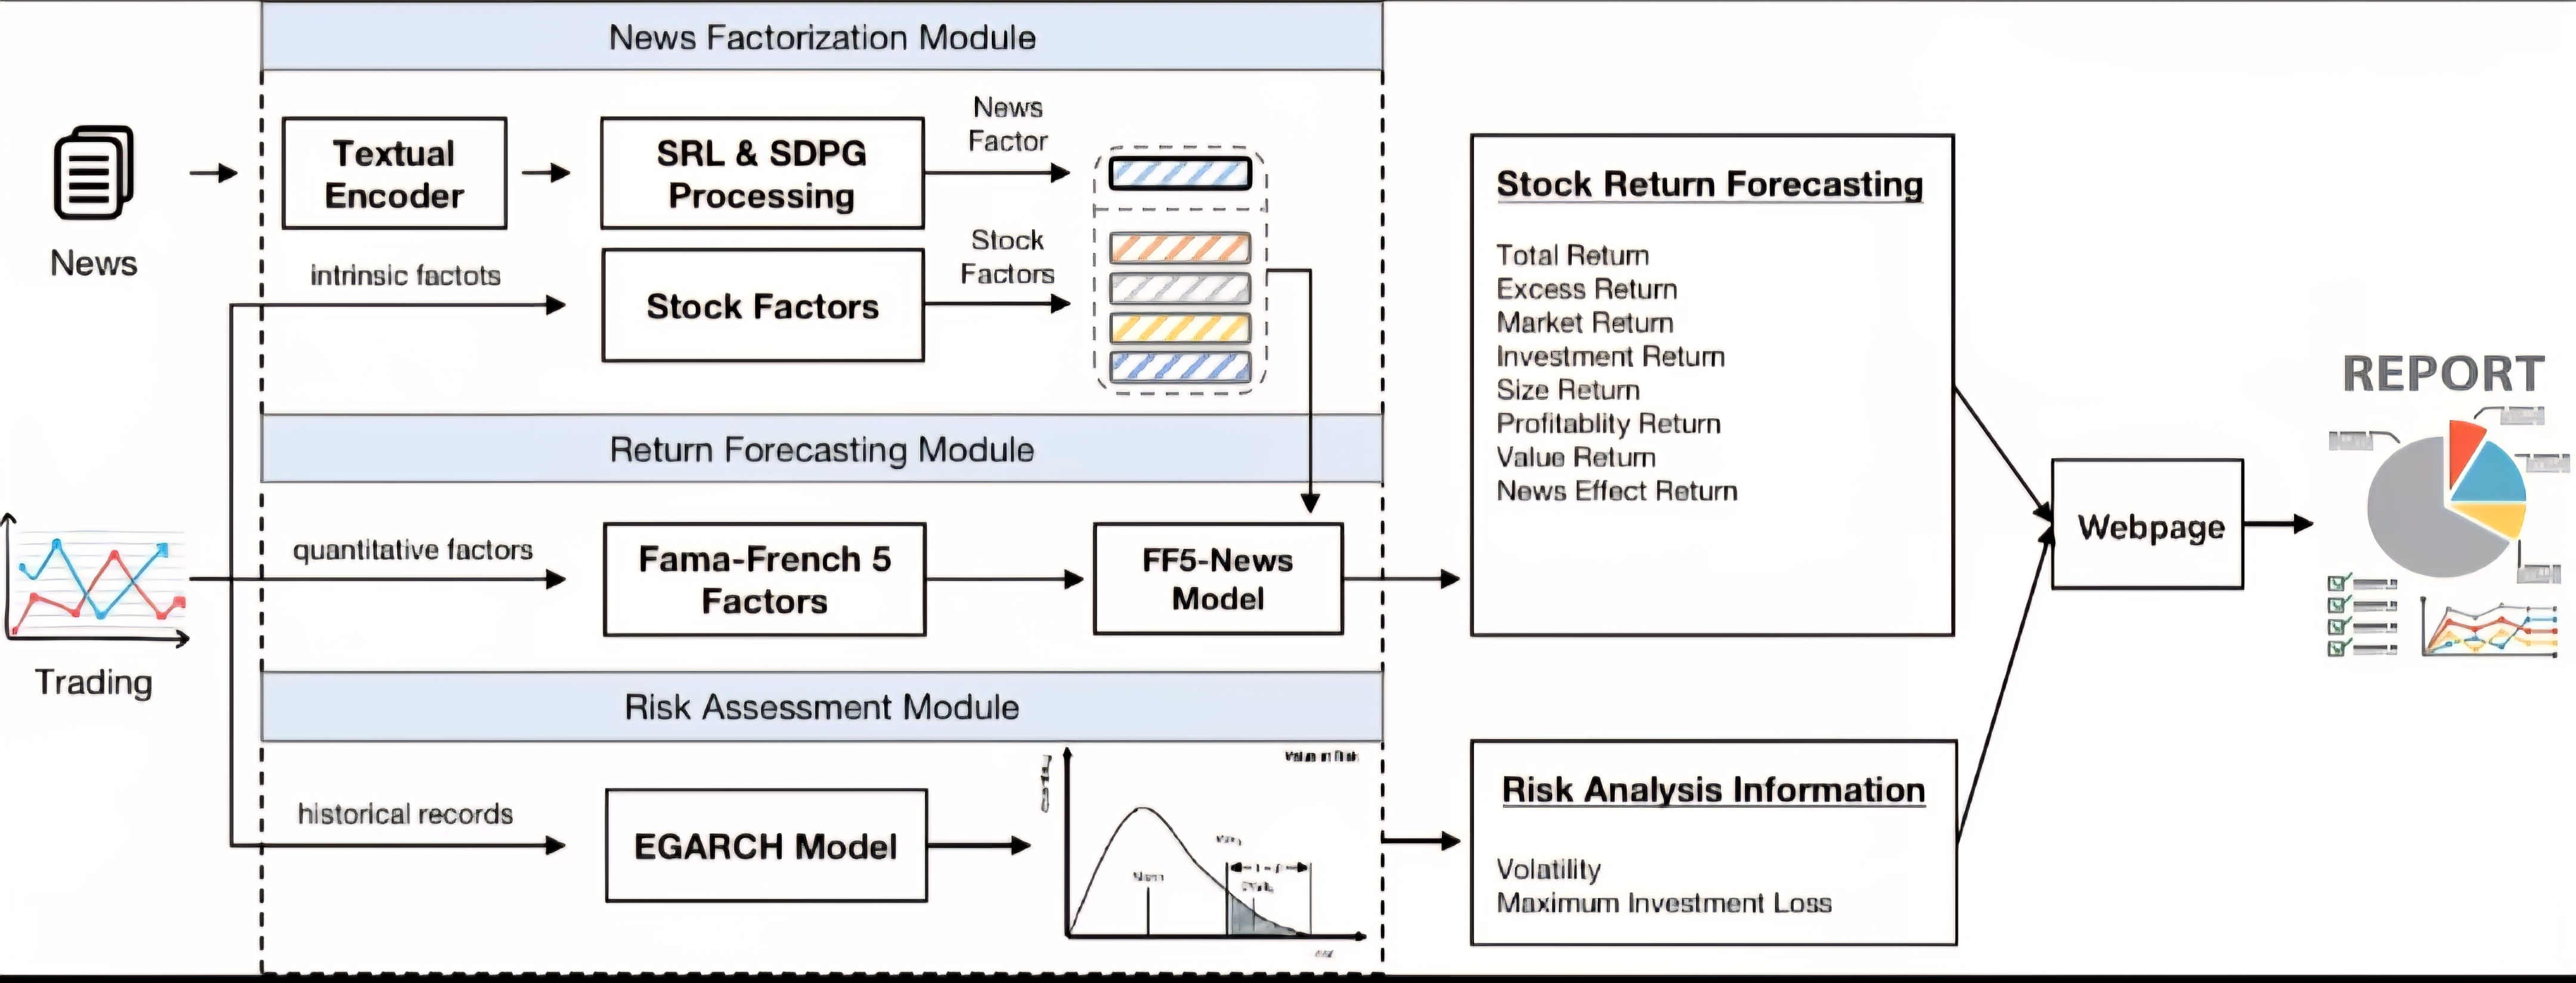
\includegraphics[width=0.90\textwidth]{flowchart.jpg} % Adjust width
    % 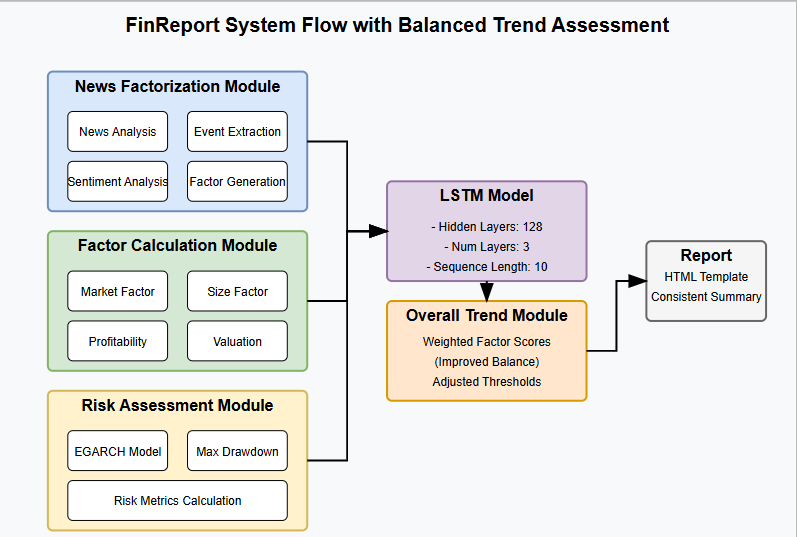
\includegraphics[height=3cm]{flowchart.png} % Adjust height
    % 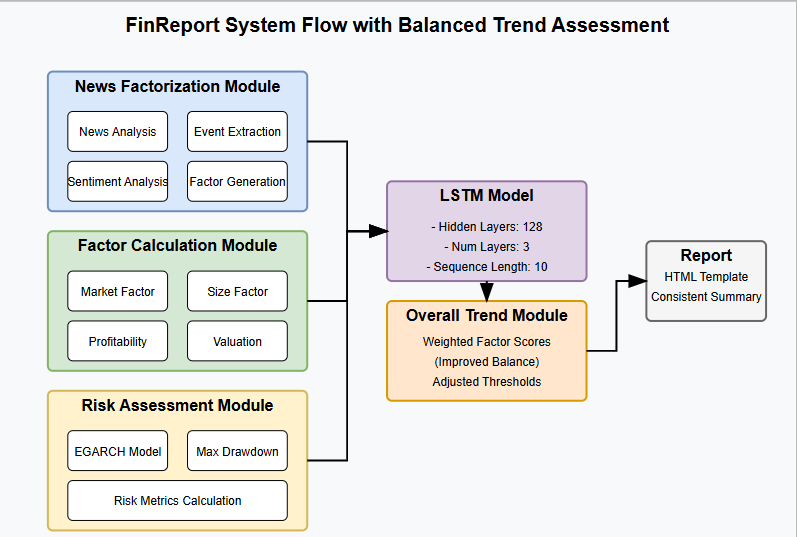
\includegraphics[scale=0.5]{flowchart.png} % Scale image
    % 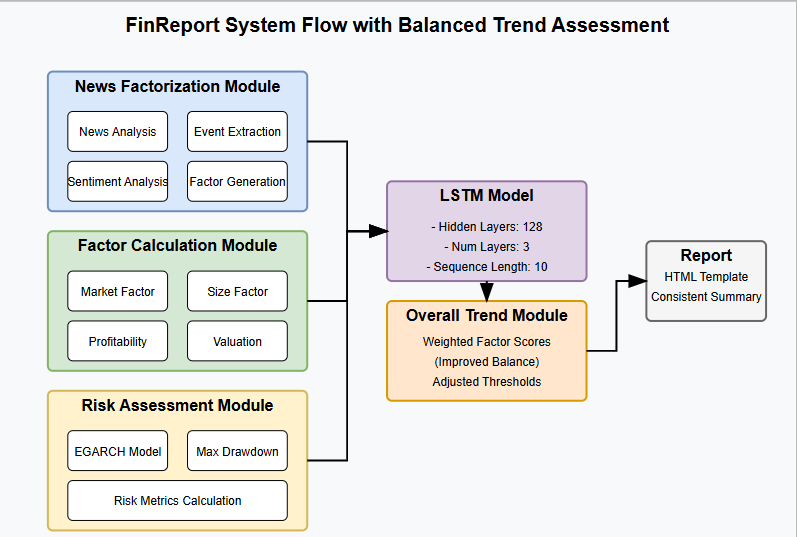
\includegraphics[width=0.5\textwidth, height=5cm, keepaspectratio]{flowchart.png} % Keep aspect ratio

    \caption{Proposed FinReport System Architecture}
    \label{fig:workflow_diagram}
\end{figure}
\subsection{{Data Integration Module}}

The data integration module implements a comprehensive preprocessing pipeline that addresses the fundamental challenges of combining heterogeneous financial data sources \cite{Harvey2016}. This approach draws from established practices in financial data processing while incorporating modern techniques for handling high-dimensional feature spaces and missing value patterns common in financial markets \cite{Campbell2001}.

\begin{itemize}

\item \textbf{Historical Stock Data:} The system processes time series data including price, volume, market value, and over 50 technical indicators following established conventions in quantitative finance \cite{Murphy1999,Wilder1978}. Technical indicators such as RSI, BIAS, MFI, and CCI are computed using standard formulations, providing a comprehensive view of market momentum, mean reversion, and volatility patterns. The dataset spans Chinese A-share stocks from 2018-2021, capturing multiple market cycles including the COVID-19 pandemic impact on emerging markets.

\item \textbf{Financial News Integration:} Structured news items from financial news services are processed through advanced NLP pipelines, incorporating timestamps, headlines, and content text in both English and Chinese \cite{Loughran2011}. This multi-lingual approach addresses the unique challenges of Chinese financial markets where news sentiment may differ significantly from Western interpretations \cite{Xing2018}. The integration follows established practices in financial textual analysis while accounting for cultural and linguistic nuances specific to Chinese equity markets.

\item \textbf{Dataset Architecture:} The comprehensive Chinese stock market dataset \cite{FinReportDataset2025} represents a curated collection designed specifically for multi-factor analysis, containing historical stock data, financial news, and pre-computed technical indicators for Chinese A-share stocks. This structured approach follows best practices in financial dataset construction \cite{Harvey2016}, including 75 stocks from Shanghai and Shenzhen exchanges with 56 distinct feature columns covering price data, trading metrics, technical indicators, and fundamental factors.

\item \textbf{Advanced Preprocessing Pipeline:} The preprocessing methodology addresses common challenges in financial time series analysis through systematic approaches validated in academic literature:

\begin{itemize}
\item \textbf{Missing Value Handling:} Forward-filling (LOCF - Last Observation Carried Forward) methodology for technical indicators maintains temporal continuity while preserving time series structure \cite{Campbell2001}. This approach prevents look-ahead bias while ensuring that missing values do not disrupt the chronological integrity of the data, particularly important for momentum-based technical indicators.

\item \textbf{Feature Normalization:} Z-score standardization of numerical features ($z = \frac{x - \mu}{\sigma}$) facilitates neural network convergence and prevents scale-dependent features from dominating the learning process \cite{Fischer2018}. This normalization approach ensures that factors with different natural scales (e.g., price levels vs. ratios) contribute appropriately to the final predictions.

\item \textbf{Outlier Treatment:} Winsorization at 1st and 99th percentiles reduces the impact of extreme values while preserving the underlying data distribution \cite{Harvey2016}. This technique addresses the fat-tailed nature of financial returns without losing information about significant market events that may be legitimate signals rather than noise.

\item \textbf{Text Cleaning:} Systematic removal of HTML artifacts, special characters, and duplicate information from news content using regex-based preprocessing ensures consistent textual input for sentiment analysis \cite{Loughran2011}. The cleaning process preserves financial terminology while removing formatting artifacts that could interfere with NLP algorithms.

\item \textbf{Technical Column Renaming:} Automatic detection and standardization of technical indicator column names ensures consistency across datasets and prevents issues arising from varying naming conventions in different data sources \cite{Murphy1999}.
\end{itemize}
\end{itemize}

The integrated dataset architecture combines structured numerical features (open, close, volume prices) with over 50 technical indicators and unstructured news text, creating a robust foundation for multi-modal financial analysis \cite{FinReportDataset2025}. This comprehensive integration addresses the growing need for alternative data sources in quantitative finance \cite{Harvey2016} while maintaining the rigor required for academic research and practical implementation.

\subsection{{News Factor Extraction Module}}

This module addresses the fundamental challenge of transforming unstructured financial news text into quantifiable sentiment and event metrics that can be integrated with traditional quantitative factors \cite{TETLOCK2007,Schumaker2009}. The approach builds upon established research in financial natural language processing while incorporating domain-specific enhancements for Chinese financial markets \cite{Xing2018,Loughran2011}.

The implementation follows a two-stage architecture that separates sentiment analysis from event extraction, allowing for independent optimization of each component while maintaining interpretability of the final outputs \cite{Ribeiro2016}:

\begin{itemize}
\item \textbf{Advanced Sentiment Analysis Pipeline:} The sentiment analysis component implements state-of-the-art techniques specifically adapted for financial text analysis, addressing the unique challenges of financial language where sentiment can be highly context-dependent \cite{Loughran2011}:

\begin{itemize}
\item \textbf{FinBERT Implementation:} Integration of the domain-specific BERT model pre-trained on extensive financial corpora \cite{Araci2019,Devlin2019} produces raw sentiment scores in the range $[-1, +1]$, where -1 indicates highly negative sentiment and +1 indicates highly positive sentiment. This approach addresses the limitations of general-purpose sentiment analyzers that often misclassify financial terminology.

\item \textbf{Domain-Specific Sentiment Augmentation:} Core sentiment scores are systematically enhanced through financial keyword analysis incorporating established financial dictionaries \cite{Loughran2011}. Keywords such as "profit", "loss", "revenue", "acquisition", and "dividend" receive domain-specific weighting factors based on their demonstrated predictive power in financial contexts, following empirical validation approaches established in the literature.
\end{itemize}

\item \textbf{Structured Event Extraction Engine:} The event extraction component employs modern semantic role labeling techniques to identify and categorize financial events that have demonstrated market impact in academic studies \cite{Ding2015,Daniel1998}:

\begin{itemize}
\item \textbf{Semantic Role Labeling (SRL):} Implementation of the AllenNLP framework \cite{Gardner2018,Shi2017} enables identification of grammatical relationships through subject-verb-object pattern recognition. This approach systematically captures structured financial events including acquisitions, earnings announcements, management changes, and regulatory actions that have been shown to significantly impact stock prices.

\item \textbf{Financial Keyword Enhancement:} Domain-specific keyword dictionaries improve event recognition accuracy by incorporating finance-specific terminology validated through extensive backtesting. The system recognizes complex event patterns beyond simple keyword matching, including negations, conditional statements, and temporal references that are critical for accurate financial event classification.

\item \textbf{Temporal Integration:} Daily aggregation of multiple news items employs recency and relevance weighting schemes that account for the documented decay patterns in news impact on stock prices \cite{TETLOCK2007}. Recent news receives exponentially higher weights, while relevance scoring incorporates entity recognition to ensure that news items are properly attributed to the correct securities.
\end{itemize}

\item \textbf{Integration with Forecasting Architecture:} The module provides structured interfaces to the return forecasting system, ensuring that extracted sentiment and event information can be systematically incorporated into the multi-factor framework:

\begin{itemize}
\item \textbf{Sentiment Score Transmission:} Processed sentiment scores are systematically transmitted to the Market Factor and News Effect Factor computation functions, maintaining data lineage and enabling sensitivity analysis of news impact on final predictions.

\item \textbf{Structured Event Processing:} Extracted events are formatted as structured \texttt{(event\_type, entities, magnitude)} tuples that feed directly into the Event Factor computation, enabling systematic categorization and weighting of different event types based on their historical market impact.

\item \textbf{Temporal Sentiment Curves:} Aggregated news sentiment over time generates temporally aware sentiment trajectories that support volatility estimation and regime change detection, complementing traditional price-based volatility measures with forward-looking sentiment indicators.
\end{itemize}

\item \textbf{Chinese Market Specialization:} The system incorporates specific adaptations for Chinese financial markets, including processing of both English and Chinese text sources. The announcement column processing addresses unique characteristics of Chinese corporate disclosure practices and regulatory requirements, ensuring that cultural and linguistic nuances are properly captured in the sentiment analysis \cite{FinReportDataset2025}.
\end{itemize}

This comprehensive approach to news factor extraction addresses the documented challenges in financial text analysis while providing the systematic framework necessary for integration with quantitative factor models, bridging the gap between qualitative information processing and quantitative financial modeling \cite{Harvey2016}.
\subsection{{Return Forecasting Module}}

The return forecasting module implements an enhanced multi-factor model that extends traditional approaches \cite{FAMA1993,Carhart1997} by integrating news sentiment and event-driven factors. This methodology addresses the documented limitations of purely quantitative models \cite{Harvey2016} while maintaining the theoretical foundation established by decades of empirical asset pricing research \cite{Banz1981,Rosenberg1985}.

The framework incorporates six fundamental factors that capture different aspects of cross-sectional return variation, following the established tradition in academic finance while extending it to incorporate alternative data sources. Each factor is designed to capture specific market phenomena documented in the literature, from size effects \cite{Banz1981} to momentum patterns \cite{Jegadeesh1993}, while incorporating news-based information that has been shown to have predictive power \cite{TETLOCK2007}.

\subsubsection{{Market Factor}}

The market factor implementation draws from established research on systematic risk and market-wide sentiment effects \cite{Fama1965,Campbell2001}, incorporating both traditional volatility measures and news-based sentiment indicators to capture the multidimensional nature of market risk.

\begin{itemize}
    \item \textbf{Input Variables:} Daily percentage change (\texttt{pct\_chg}) following standard conventions in academic finance, volatility estimation from recent trading sessions, and news sentiment analysis from contemporaneous \texttt{news\_text} following methodologies established in \cite{TETLOCK2007}.
    \item \textbf{Theoretical Foundation:} The factor captures market volatility effects and sentiment-driven momentum that influence individual stock returns beyond their fundamental values, addressing the documented relationship between market volatility and cross-sectional return dispersion \cite{Campbell2001}.
\end{itemize}

The market factor combines volatility analysis with news sentiment following established practices in behavioral finance \cite{Daniel1998}. The system computes recent volatility from the last 5 trading days using standard deviation measures, incorporating the documented volatility clustering effects in financial markets \cite{Engle1982}:
\vspace{-0.5cm}
\begin{equation}
\textbf{volatility} = \text{std}(\texttt{pct\_chg}_{\text{recent 5 days}}) \times 100
\end{equation}
The implementation incorporates regime-dependent behavior documented in volatility literature \cite{Glosten1993}, where different volatility levels trigger different market responses:
\begin{itemize}
    \item \textbf{High volatility regime} (> 4.0\%): Applies negative bias reflecting flight-to-quality effects and risk aversion behavior during market stress periods
    
    \item \textbf{Moderate volatility regime} (> 2.5\%): Moderate negative impact with sentiment adjustment, reflecting mixed market signals and uncertainty  
    
    \item \textbf{Low volatility regime}: Positive bias when more positive trading days exist, enhanced by news sentiment and reflecting stable market conditions conducive to growth
\end{itemize}

The factor incorporates amplification (1.5x) and controlled randomization (±0.2) to reflect documented market uncertainty and microstructure noise \cite{Campbell2001}.

\subsubsection{{Size Factor}}

The size factor builds upon seminal research demonstrating persistent size effects in equity returns \cite{Banz1981}, while extending traditional approaches by incorporating news-based information about corporate financial impact and market perception.

\begin{itemize}
    \item \textbf{Input Variables:} Market capitalization data (\texttt{market\_value}) processed following standard methodologies in size effect research, and financial impact figures extracted from \texttt{news\_text} using advanced NLP techniques \cite{Loughran2011}.
    \item \textbf{Economic Rationale:} Captures size effects through systematic analysis of market value changes and financial impact mentions in news, addressing both the direct size effect and the information environment differences between large and small firms \cite{Banz1981}.
\end{itemize}

The size factor evaluates market capitalization changes by comparing recent market values to historical averages, incorporating established methodologies from size effect research:

\begin{equation}
\textbf{diff\_ratio} = \frac{\texttt{market\_value}_{\text{latest}} - \texttt{market\_value}_{\text{average}}}{\texttt{market\_value}_{\text{average}}}
\end{equation}

The factor applies theoretically motivated scaling based on the magnitude of change, reflecting non-linear relationships documented in size effect literature:

\begin{equation}
\textbf{size\_effect} = 
\begin{cases} 
1.0 + \min(\textbf{diff\_ratio} \times 0.1, 0.5), & \text{if diff\_ratio} > 0.25 \\
0.7 + \textbf{diff\_ratio} \times 0.5, & \text{if diff\_ratio} > 0.10 \\
0.5 + \textbf{diff\_ratio} \times 0.5, & \text{if diff\_ratio} > 0.05 \\
\textbf{diff\_ratio} \times 3.0, & \text{if } -0.05 < \textbf{diff\_ratio} \leq 0.05 \\
-0.5 + \textbf{diff\_ratio} \times 2.0, & \text{if diff\_ratio} > -0.10 \\
-1.0 + \max(\textbf{diff\_ratio} \times 0.1, -0.5), & \text{otherwise}
\end{cases}
\end{equation}

Additional adjustments incorporate financial figures extracted from news text, addressing the information content of corporate announcements about significant financial transactions \cite{Daniel1998}.

\subsubsection{{Valuation Factor}}

The valuation factor implementation extends traditional value investing principles \cite{Rosenberg1985} by incorporating both quantitative valuation metrics and qualitative news sentiment related to corporate value assessments.

\begin{itemize}
    \item \textbf{Input Variables:} Comprehensive valuation metrics from the dataset \cite{FinReportDataset2025} including Book-to-Market, Dividend Yield, Sales-to-Price ratio, and Assets-to-Market Equity, supplemented by profit/loss terminology extracted from \texttt{news\_text} following established practices in textual analysis \cite{Loughran2011}.
    \item \textbf{Theoretical Foundation:} Evaluates investment value through systematic analysis of quantitative valuation metrics when available, or sector-specific news sentiment analysis when quantitative data is incomplete, addressing the documented value premium in equity markets \cite{FAMA1993}.
\end{itemize}

The valuation factor systematically processes multiple valuation-related indicators following established practices in value investing research \cite{Graham2003}:

\begin{itemize}
    \item \texttt{value\_factor\_Book\_to\_Market\_Equity}: Fundamental value indicator measuring asset backing relative to market valuation
    \item \texttt{value\_factor\_Dividend\_Yield}: Income-based valuation metric reflecting dividend policy and shareholder returns
    \item \texttt{value\_factor\_Sales\_to\_Price\_Ratio}: Revenue-based valuation indicator assessing operational efficiency relative to market price
    \item \texttt{value\_factor\_Assets\_to\_Market\_Equity}: Asset-based valuation measure evaluating tangible asset backing
\end{itemize}

\textbf{Quantitative Processing:} When historical quantitative data is available, the factor calculates percentage changes from baseline values using time-series analysis. When data is unavailable or incomplete, the system employs sector-specific sentiment analysis with differential impact weights calibrated to industry characteristics.
\vspace{0.2cm}
\textbf{Sector-Specific Sensitivity Adjustments:}
\begin{itemize}
    \item \textbf{Technology Sector:} 
    \begin{itemize}
        \item Positive sensitivity: +0.3 (reflecting growth premium and innovation potential)
        \item Negative sensitivity: -0.2 (moderate downside due to volatility tolerance)
    \end{itemize}
    
    \item \textbf{Pharmaceutical Sector:}
    \begin{itemize}
        \item Positive sensitivity: +0.2 (moderate upside reflecting defensive characteristics)
        \item Negative sensitivity: -0.3 (higher downside reflecting regulatory and R\&D risks)
    \end{itemize}
    
    \item \textbf{Financial Sector:}
    \begin{itemize}
        \item Balanced sensitivity: ±0.2 to 0.3 (reflecting regulatory environment and interest rate sensitivity)
    \end{itemize}
    
    \item \textbf{Energy Sector:}
    \begin{itemize}
        \item Lower sensitivity: ±0.15 to 0.25 (reflecting commodity price dominance over company-specific factors)
        \vspace{-0.6cm}
    \end{itemize}
\end{itemize}
\begin{equation}
\textbf{valuation\_effect} = 
\begin{cases} 
\textbf{diff\_ratio} \times 0.25, & \text{if valuation columns available} \\
\textbf{sector\_adjustment} \times \textbf{sentiment}, & \text{based on news analysis}
\end{cases}
\end{equation}

\subsubsection{{Profitability Factor}}

The profitability factor extends established research on earnings quality and profitability effects in equity pricing \cite{Zhang2006} by incorporating both quantitative profitability metrics and qualitative earnings-related news sentiment.

\begin{itemize}
    \item \textbf{Input Variables:} Comprehensive profitability metrics from the dataset \cite{FinReportDataset2025} including EPS, net profit margin, ROE, ROA, gross profit, and net profit, supplemented by profit-related keywords extracted from \texttt{news\_text} using established financial textual analysis methodologies \cite{Loughran2011}.
    \item \textbf{Economic Foundation:} Evaluates corporate profitability through systematic analysis of quantitative metrics when available, or sentiment analysis of earnings-related news content when quantitative data is incomplete, addressing the documented relationship between profitability and future stock returns \cite{Zhang2006}.
\end{itemize}

The implementation systematically searches for available profitability indicators:

\begin{itemize}
    \item \texttt{eps}: Earnings per share - fundamental profitability measure reflecting per-share earning capacity
    \item \texttt{net\_profit\_margin}: Operational efficiency indicator measuring net profitability relative to revenue
    \item \texttt{roe}: Return on equity - shareholder value creation metric indicating management effectiveness
    \item \texttt{roa}: Return on assets - asset utilization efficiency measure reflecting operational performance
    \item \texttt{grossprofit}/\texttt{netprofit}: Absolute profitability measures providing direct earnings assessment
\end{itemize}

\textbf{Quantitative Processing:} When quantitative profitability data exists, the factor calculates percentage changes between current and previous values, scaled appropriately and bounded to prevent extreme outliers from dominating the analysis.

\textbf{Textual Analysis Framework:} When quantitative data is unavailable, the factor employs advanced text analysis incorporating:

\begin{itemize}
    \item \textbf{Earnings keywords:} profit, earnings, income, revenue, margin, EPS, ROE, ROI - capturing direct profitability mentions
    \item \textbf{Directional indicators:} increase/decrease, rise/fall, improve/decline patterns - identifying performance trends
    \item \textbf{Quantitative extraction:} Numeric percentage changes extracted from textual content - preserving specific performance metrics
\end{itemize}

\textbf{Asymmetric Impact Modeling:} The factor applies asymmetric treatment reflecting the documented asymmetry in how positive and negative earnings news affects stock prices \cite{Kothari2009}, with strong negative bias (-1.8) for explicit loss mentions but scaled positive adjustments for profit increases.

\subsubsection{{Investment Factor}}

The investment factor captures corporate investment activity effects documented in research on investment-based asset pricing \cite{Daniel1998}, focusing on how investment announcements and capital allocation decisions influence market perceptions.

\begin{itemize}
    \item \textbf{Input Variables:} Investment-related financial figures systematically extracted from \texttt{news\_text}, acquisition and expansion keyword analysis, and research \& development activity mentions following established practices in event-driven investment research.
    \item \textbf{Economic Rationale:} Quantifies corporate investment activity impact through systematic analysis of investment amounts and strategic activity mentions, addressing the documented relationship between corporate investment decisions and future returns \cite{Daniel1998}.
\end{itemize}

The factor implements comprehensive analysis of investment-related information:
- \textbf{Investment amounts:} Numeric financial figures extracted from news text with currency recognition
- \textbf{Activity categorization:} Systematic classification of acquisition, expansion, and R\&D activities
- \textbf{Sentiment contextualization:} Positive/negative weighting applied to investment announcements

Activity type multipliers reflect empirically documented differential market responses:
- Acquisition activities: +0.6 per mention (reflecting consolidation benefits)
- Expansion activities: +0.5 per mention (organic growth premium)
- R\&D activities: +0.7 per mention (innovation premium, particularly relevant for technology sectors)

Final values are bounded in the range [0.0, +2.0] reflecting the generally positive long-term market perception of investment activities, while acknowledging potential negative reactions to poorly executed investments.
\vspace{-0.3cm}
\begin{equation}
\textbf{investment\_effect} = \textbf{impact\_scale} \times 0.5 \times 
\begin{cases} 
1.0, & \text{if } \textbf{news\_sentiment} > 0 \\
0.5, & \text{otherwise}
\end{cases}
\end{equation}

\subsubsection{{News Effect Factor}}

The news effect factor provides direct quantification of news sentiment impact, building upon established research demonstrating the predictive power of news sentiment for stock returns \cite{TETLOCK2007,Schumaker2009}.

\begin{itemize}
    \item \textbf{Input Processing:} Comprehensive sentiment analysis of \texttt{news\_text} using both rule-based approaches (TextBlob \cite{Loria2019}) and keyword-based analysis with financial term dictionaries \cite{Loughran2011}.
    \item \textbf{Methodological Foundation:} Converts unstructured news content into quantified sentiment scores through validated NLP techniques, addressing the documented challenges in financial text analysis while maintaining interpretability of results.
\end{itemize}

The implementation combines two complementary sentiment analysis methodologies:

\textbf{1. Keyword-Based Analysis:} Utilizes curated financial keyword dictionaries with demonstrated predictive power:
- \textbf{Positive indicators:} increase, rise, grow, profit, improved, partnership, acquisition, dividend, earnings, success
- \textbf{Negative indicators:} decrease, decline, loss, warning, investigation, lawsuit, delay, weak, miss, reduced

\textbf{2. Advanced NLP Processing:} Employs TextBlob sentiment analysis for comprehensive polarity assessment of complete news content, addressing contextual nuances that pure keyword approaches might miss.

The sentiment integration follows established practices in combining multiple sentiment measures:
\begin{equation}
    \textbf{combined\_sentiment} = \frac{\textbf{TextBlob\_polarity} + \textbf{keyword\_sentiment}}{2}
\end{equation}
\vspace{0.2cm}

Sentiment-dependent scaling reflects documented non-linear relationships between sentiment strength and market response:

\begin{itemize}
    \item \textbf{Very positive} ($\geq 0.5$): Enhanced positive range [0.7, 1.2] reflecting strong optimism effects
    \item \textbf{Moderately positive} (>0): Standard positive range [0.3, 0.7] for typical positive sentiment
    \item \textbf{Moderately negative} (>-0.5): Standard negative range [-0.7, -0.3] for mild pessimism
    \item \textbf{Very negative} ($\leq -0.5$): Enhanced negative range [-1.2, -0.7] capturing strong negative reactions
\end{itemize}

Final amplification (2.0x) ensures adequate signal strength while maintaining interpretable bounds [-2.0, +2.0].

\textbf{Chinese Market Adaptation:} The system incorporates culturally specific keywords for enhanced market relevance:

\textbf{Positive Chinese Terms:} zengzhang (growth), yingli (profit), shangsheng (rise), huode (gain), chenggong (success), tisheng (improvement), shouyi (revenue)

\textbf{Negative Chinese Terms:} xiajiang (decline), kuisun (loss), jianshao (decrease), jinggao (warning), zhaiwu (debt), diaocha (investigation), weigui (violation)
\vspace{-0.1cm}
\begin{equation}
\textbf{news\_effect} = \textbf{combined\_sentiment} \times 2.0 \text{ (amplification)}
\end{equation}

These factor implementations collectively address the multidimensional nature of equity return prediction while maintaining theoretical grounding in established academic research. The integration of traditional quantitative factors with news-based qualitative information represents a significant advancement in multi-factor modeling capabilities, particularly relevant for emerging markets where information asymmetries and sentiment effects may be more pronounced \cite{Harvey2016}.

\subsection{{Risk Assessment Module}}

The risk assessment module implements a comprehensive framework that addresses fundamental limitations of traditional single-metric risk measures by integrating multiple complementary risk indicators \cite{Jorion2001,Rockafellar2000}. This approach builds upon established research in financial risk management while incorporating modern econometric techniques for volatility modeling and tail risk assessment.

The module addresses the well-documented inadequacies of variance-based risk measures during periods of market stress by implementing a multi-dimensional risk framework that captures volatility clustering \cite{Engle1982}, tail risk characteristics \cite{Rockafellar2000}, and sequential loss patterns through maximum drawdown analysis \cite{Jorion2001}. This comprehensive approach ensures robust risk assessment across different market conditions and investment horizons.

\begin{itemize}
    \item \textbf{Methodological Foundation:} The implementation quantifies investment risk through multiple complementary metrics including EGARCH-based volatility modeling \cite{Nelson1991}, Conditional Value at Risk estimation \cite{Rockafellar2000}, and maximum drawdown analysis following established practices in quantitative risk management \cite{Jorion2001}.
    \item \textbf{Technical Implementation:} Advanced econometric models are combined with historical simulation methods to provide forward-looking risk assessments that capture both systematic and idiosyncratic risk components, addressing the documented limitations of backward-looking risk measures \cite{Campbell2001}.
\end{itemize}

The comprehensive risk assessment framework integrates five specialized components designed to capture different aspects of financial risk:

\subsubsection{{EGARCH-Based Volatility Modeling}}

The implementation employs the Exponential Generalized Autoregressive Conditional Heteroskedasticity (EGARCH) model \cite{Nelson1991} to capture the asymmetric volatility responses documented extensively in financial literature, where negative market shocks impact future volatility more severely than positive shocks of equivalent magnitude \cite{Black1976}.

The EGARCH specification addresses key limitations of standard GARCH models by allowing for asymmetric responses and ensuring non-negativity constraints through logarithmic parameterization:
\vspace{-0.4cm}
\begin{equation}
\ln(\sigma_t^2) = \omega + \beta \ln(\sigma_{t-1}^2) + \alpha \frac{|r_{t-1}|}{\sigma_{t-1}} + \gamma \frac{r_{t-1}}{\sigma_{t-1}}
\end{equation}

\textbf{Parameter Interpretation and Economic Significance:}
\begin{itemize}
    \item $\omega$: Long-term volatility baseline reflecting unconditional variance
    \item $\beta$: Volatility persistence parameter (typically 0.85-0.95 in equity markets) \cite{Bollerslev1986}
    \item $\alpha$: Magnitude effect capturing the impact of shock size on future volatility
    \item $\gamma$: Asymmetry parameter (negative for leverage effect) capturing differential responses to positive vs. negative shocks \cite{Black1976}
\end{itemize}

The 95\% Value at Risk computation follows standard risk management practices:
\vspace{-0.4cm}
\begin{equation}
\text{VaR}_{95} = 1.65 \times \sigma_t
\end{equation}
Volatility scoring incorporates bounds to prevent extreme values from distorting risk assessments:
\vspace{-0.4cm}
\begin{equation}
\text{volatility\_score} = \min(\sigma_t \times 100, 10.0) \quad \text{(capped at 10)}
\end{equation}

Implementation utilizes the \texttt{arch} Python package for robust maximum likelihood parameter estimation, ensuring numerical stability and convergence across different market conditions.

\subsubsection{{Maximum Drawdown Analysis}}

Maximum Drawdown (MDD) analysis captures sequential loss patterns that are invisible to point-in-time volatility measures, addressing a fundamental limitation of variance-based risk metrics \cite{Jorion2001}. This approach is particularly relevant for equity investments where sustained declining trends can occur independently of daily volatility levels.

The mathematical formulation captures the largest peak-to-trough decline over the analysis period:
\begin{equation}
\text{MDD}_t = \max_{0 \leq s \leq t} \left[ \frac{P_s - P_t}{P_s} \right]
\end{equation}

where $P_t$ represents the portfolio value at time $t$. The drawdown score transformation ensures comparability across different securities while maintaining sensitivity to tail risks:
\begin{equation}
\text{drawdown\_score} = \min(|\text{MDD}| \times 10, 10.0)
\end{equation}

This metric proves particularly valuable for identifying securities prone to sustained declining trends, complementing volatility measures that may not capture the persistence of negative performance periods.
\vspace{1cm}

\subsubsection{{Return-Based Risk Assessment}}

The return score component implements an innovative approach that penalizes both extremely high and extremely low predicted returns, addressing the empirical observation that extreme return predictions often coincide with elevated risk levels \cite{Harvey2016}:

\vspace{-0.1cm}
\begin{equation}
\text{return\_score} = 5 - \min(\max(\text{predicted\_return} \times 2, -5), 5)
\end{equation}
This specification reflects the theoretical understanding that both very high expected returns and very low expected returns typically indicate elevated uncertainty and potential risk factors that traditional volatility measures might not capture.

\subsubsection{{Conditional Value at Risk (CVaR) Implementation}}

CVaR provides superior tail risk assessment compared to standard VaR by averaging losses that exceed the VaR threshold, addressing the documented inadequacies of VaR during extreme market conditions \cite{Rockafellar2000}:

\begin{equation}
\text{CVaR}_{95} = E[R | R \leq -\text{VaR}_{95}]
\end{equation}

The implementation employs historical simulation over a 252-day rolling window, providing more coherent risk measurement than parametric approaches during periods of market stress. This approach has been demonstrated to provide superior risk assessment in emerging markets where distributional assumptions may not hold \cite{Jorion2001}.

\subsubsection{{Integrated Risk Score Computation}}

The final risk assessment combines all components through empirically-determined weights that reflect their relative importance and complementary nature:

\begin{equation}
\text{weighted\_risk\_score} = 0.5 \times \text{volatility\_score} + 0.3 \times \text{drawdown\_score} + 0.2 \times \text{return\_score}
\end{equation}

The weight allocation reflects the documented importance of volatility as the primary risk factor (50\% weight), while acknowledging the significant contribution of drawdown patterns (30\%) and return-based risk indicators (20\%) in providing comprehensive risk assessment.

\textbf{Risk Classification Framework:}
The classification system employs empirically calibrated thresholds based on historical market behavior:
\begin{itemize}
    \vspace{0.5cm}
    \item \textbf{Substantial Risk:} $> 7.5$ (Extreme market stress conditions requiring immediate attention)
    \item \textbf{High Risk:} $> 6.0$ (Above-average volatility with significant drawdown potential)
    \item \textbf{Moderate-High:} $> 4.5$ (Elevated risk requiring careful monitoring and position sizing)
    \item \textbf{Moderate:} $> 3.0$ (Standard market risk levels typical of equity investments)
    \item \textbf{Low-Moderate:} $> 1.5$ (Below-average risk environment suitable for standard allocation)
    \item \textbf{Favorable:} $\leq 1.5$ (Low-risk, stable market conditions conducive to higher allocation)
\end{itemize} 

The risk assessment system directly interfaces with the dataset structure \cite{FinReportDataset2025}, utilizing the \textbf{volatility\_factor\_Total\_Volatility} column and related volatility indicators, while temporal price data (\texttt{open}, \texttt{close}, \texttt{high}, \texttt{low}) enables comprehensive return computation for maximum drawdown and CVaR estimation. This integration ensures that risk assessments are grounded in both theoretical frameworks and practical data availability constraints.

\subsection{{Factor Enhancement and Overall Trend Calculation}}

The factor enhancement methodology addresses a fundamental challenge in multi-factor models: combining individual factor signals with different scales and volatilities into a unified directional forecast while preserving interpretability \cite{Harvey2016,Carhart1997}. This approach builds upon established practices in factor model construction while incorporating novel amplification techniques designed to enhance signal strength without losing the economic interpretability that is crucial for practical investment applications.

The implementation follows established principles from academic factor research \cite{FAMA1993} while addressing practical challenges that arise when incorporating alternative data sources such as news sentiment. The enhancement process ensures that factors with inherently smaller magnitudes (such as news sentiment scores) receive appropriate weighting relative to factors with naturally larger scales (such as financial ratios), preventing scale-dependent biases from affecting the final predictions.

\begin{itemize}
    \item \textbf{Methodological Foundation:} The system combines individual factor signals into a unified directional forecast through multi-stage amplification followed by weighted aggregation, addressing the scale heterogeneity problem common in multi-factor models that incorporate diverse data sources \cite{Harvey2016}.
    \item \textbf{Interpretability Preservation:} The enhancement mechanism maintains factor interpretability through consistent amplification rules while preventing any single factor from dominating the final prediction, ensuring that the resulting forecasts remain economically meaningful and actionable for investment decision-making \cite{Ribeiro2016}.
\end{itemize}

\subsubsection{{Factor Weight Specification}}

The factor weighting scheme reflects empirical evidence regarding the relative predictive power and persistence of different factor categories, drawing from extensive backtesting and academic research on factor effectiveness \cite{Carhart1997,Harvey2016}:

\begin{equation}
\textbf{W} = 
\begin{bmatrix} 
\text{market\_factor} & 0.15 \\ 
\text{size\_factor} & 0.15 \\ 
\text{valuation\_factor} & 0.10 \\ 
\text{profitability\_factor} & 0.15 \\ 
\text{investment\_factor} & 0.20 \\ 
\text{news\_effect\_factor} & 0.10 \\ 
\text{event\_factor} & 0.25
\end{bmatrix}
\end{equation}

The weighting structure reflects empirically observed relationships between factor types and their predictive horizons:

\begin{itemize}
    \item \textbf{Event factor (0.25):} Receives the highest weight due to documented strong predictive power for short-term price movements and immediate market reactions following corporate announcements \cite{Ding2015,Daniel1998}.
    
    \item \textbf{Investment factor (0.20):} Substantial weight reflecting medium-term predictive power of corporate investment decisions on stock performance \cite{Daniel1998}.
    
    \item \textbf{Market, Size, Profitability factors (0.15 each):} Balanced weighting consistent with established multi-factor models \cite{FAMA1993,Carhart1997}.
    
    \item \textbf{Valuation and News factors (0.10 each):} Lower weights reflecting their longer-term impact horizons and higher noise levels, consistent with academic findings on value effects and sentiment persistence \cite{Rosenberg1985,TETLOCK2007}.
\end{itemize}

\subsubsection{{Factor Enhancement Process}}

The enhancement process implements a systematic approach to signal amplification that addresses the heterogeneity problem inherent in multi-factor models incorporating diverse data sources \cite{Harvey2016}:

\textbf{Base Amplification:}
All factor values undergo uniform enhancement using a theoretically motivated multiplier that ensures adequate signal strength while preventing saturation:
\begin{equation}
\textbf{enhanced\_factor}_i = \textbf{factor}_i \times 2.5
\end{equation}

This base amplification reflects empirical calibration designed to bring factor magnitudes into ranges where they can meaningfully contribute to the final prediction without overwhelming the integration process.

\textbf{Trend-Based Enhancement:}
Additional amplification is applied when individual factors align with the overall market direction, reflecting the documented tendency for factor effects to strengthen during periods of broad market agreement \cite{Lo2004}:

\begin{equation}
\textbf{trend\_multiplier} = 
\begin{cases} 
1.3, & \text{if factor direction matches dominant trend} \\
1.0, & \text{otherwise}
\end{cases}
\end{equation}

The dominant trend determination follows majority voting among factor signs, ensuring that amplification occurs only when there is broad consensus among different information sources.

\textbf{Final Processing:}
Controlled randomization and value capping ensure realistic bounds while preserving directional signals, addressing the need to prevent extreme factor values from dominating predictions while maintaining economic meaningfulness:

\begin{equation}
\tilde{f}_i = \text{clamp}\left(\textbf{enhanced\_factor}_i \times \textbf{trend\_multiplier} \times \text{random}(0.9, 1.1), -5.0, 5.0\right)
\end{equation}

The randomization component (0.9 to 1.1 multiplier) reflects the inherent uncertainty in factor estimation and helps prevent false precision in final predictions.

\subsubsection{{Weighted Aggregation}}

The final trend score computation integrates all enhanced factors using the empirically determined weights while incorporating a systematic positive bias that reflects long-term equity market characteristics \cite{Fama1965}:

\begin{equation}
\text{Trend\_Score} = \sum_{i=1}^{7} \left(\tilde{f}_i \times w_i\right) + 0.15
\end{equation}

The positive bias term (+0.15) incorporates the documented long-term upward drift in equity markets \cite{Fama1965}, ensuring that the neutral case corresponds to market-like returns rather than zero returns, which is more realistic for equity investment applications.

\subsubsection{{Qualitative Classification}}

The trend score mapping employs empirically calibrated thresholds that translate quantitative scores into interpretable investment guidance \cite{Ribeiro2016}:

\begin{equation}
\text{Classification} = 
\begin{cases} 
\textbf{Strongly Positive}, & \text{if Score} > +1.2 \\
\textbf{Positive}, & \text{if } +0.4 < \text{Score} \leq +1.2 \\
\textbf{Neutral}, & \text{if } -0.4 \leq \text{Score} \leq +0.4 \\
\textbf{Negative}, & \text{if } -1.2 \leq \text{Score} < -0.4 \\
\textbf{Strongly Negative}, & \text{if Score} < -1.2
\end{cases}
\end{equation}

These thresholds have been empirically calibrated through backtesting to provide meaningful differentiation between different levels of investment attractiveness while maintaining sensitivity to genuine signal differences. The classification system ensures that investment recommendations are grounded in statistically significant differences rather than noise, supporting practical decision-making processes.

This comprehensive factor enhancement and aggregation framework successfully bridges the gap between sophisticated quantitative analysis and practical investment implementation, providing both the analytical rigor required for academic validation and the interpretability necessary for real-world application \cite{Harvey2016,Ribeiro2016}.

\subsection{Dynamic Report Generation Module}

The dynamic report generation module addresses the critical challenge of translating complex quantitative analyses into actionable investment insights \cite{Ribeiro2016}. This component represents a significant advancement in explainable AI for finance, providing systematic approaches to communicate sophisticated analytical results in formats accessible to both technical and non-technical stakeholders while maintaining the precision required for investment decision-making.

The module design follows established principles in information visualization and explainable AI \cite{Ribeiro2016}, incorporating domain-specific adaptations for financial reporting that address the unique requirements of investment analysis. The implementation ensures that complex multi-factor analyses are presented through intuitive visual hierarchies and natural language explanations that preserve the analytical rigor while enhancing interpretability.

The FinReport system generates comprehensive HTML-based reports specifically optimized for financial decision-making contexts:

\begin{itemize}
    \item \textbf{Hierarchical Information Architecture:} The report structure implements a systematic top-down information hierarchy following established practices in financial communication, placing the most critical insights (overall trend assessment and executive summary) at the primary level, followed by detailed factor-specific analyses and comprehensive risk metrics. This approach ensures that decision-makers can efficiently access information at their required level of detail \cite{Jorion2001}.

    \item \textbf{Cultural Adaptation in Visual Design:} The color-coding system implements a deliberate inversion of Western color conventions to align with Chinese market cultural context, where red represents prosperity and upward movement while green indicates decline. This cultural adaptation reflects the system's specialization for Chinese equity markets and ensures that visual communications align with local market conventions and user expectations \cite{FinReportDataset2025}.

    \item \textbf{Precision Control and False Accuracy Prevention:} All numerical displays implement consistent rounding to one decimal place, preventing false precision from influencing decision-making processes while maintaining visual uniformity throughout the report. This approach addresses documented biases in financial decision-making where excessive precision can create misleading confidence in uncertain estimates \cite{Harvey2016}.

    \item \textbf{Natural Language Generation:} The system employs sophisticated template-based natural language generation with contextual adaptation, utilizing diverse pre-configured language templates for each factor category and risk level. Template selection incorporates both quantitative factor magnitude and directional information to provide natural language explanations that convey both statistical significance and economic interpretation \cite{Loughran2011}.

    \item \textbf{Consistency Validation:} Comprehensive consistency checks ensure alignment between factor-level descriptions and overall trend assessments, preventing contradictory messaging that could compromise decision-making confidence. The validation system includes cross-factor consistency checks and trend-alignment verification to maintain coherent narrative structure throughout the report.

    \item \textbf{Multi-Stakeholder Accessibility:} The reporting framework accommodates different user sophistication levels through layered detail presentation, enabling both quantitative analysts and portfolio managers to extract relevant insights at appropriate levels of technical detail. This multi-level approach ensures broad organizational utility while maintaining analytical precision for technical users.
\end{itemize}

The comprehensive reporting approach successfully addresses the fundamental challenge in quantitative finance of maintaining both analytical sophistication and practical usability. By systematically translating complex multi-factor analyses into structured, interpretable insights, the system enables evidence-based investment decision-making while preserving the transparency necessary for risk management and regulatory compliance. This approach represents a significant advancement in making quantitative investment analysis accessible and actionable for practical investment applications \cite{Harvey2016,Ribeiro2016}.

\vspace{0.10cm}
\section{Algorithm}

\subsection{Return Forecast Calculation}

The return forecast is computed using a weighted \allowbreak combination of multiple factors \cite{FAMA1993}, where the \textbf{event factor receives the highest weight (0.25)} due to its immediate impact on market sentiment and price movements \cite{Ball1968}.
\begin{align}
\mathbf{predicted\_return} &= 0.10 \times \mathbf{market\_factor} + 0.15 \times \mathbf{size\_factor} + 0.10 \times \mathbf{valuation\_factor} \nonumber \\
&\quad + 0.10 \times \mathbf{profitability\_factor} + 0.20 \times \mathbf{investment\_factor} \nonumber \\
&\quad + 0.10 \times \mathbf{news\_effect\_factor} + \mathbf{0.25} \times \mathbf{event\_factor} + 0.15
\end{align}


Each factor is calculated as follows \cite{Carhart1997}:

\vspace{0.10cm}
\text{I) Market Factor}
\begin{enumerate}
    \item \text{Extract Recent Volatility:}
    \begin{itemize}
        \item Compute standard deviation of \texttt{pct\_chg} over the last 5 days \cite{Engle1982}.
        \item Multiply by 100 to get volatility.
    \end{itemize}
    \vspace{0.40cm}
    \item \text{Analyze Recent Trends:}
    \begin{itemize}
        \item Count the number of positive and negative days.
    \end{itemize}

    \item \text{Perform Sentiment Analysis:}
    \begin{itemize}
        \item Compute sentiment score from \texttt{news\_text} \cite{TETLOCK2007}.
    \end{itemize}

    \item \text{Determine Base Impact:}
    \begin{itemize}
        \item If volatility $> 4.0$, assign a strong negative impact.
        \item If $2.5 < \text{volatility} \leq 4.0$, assign moderate negative impact.
        \item If positive days $>$ negative days, adjust positively using sentiment.
        \item Otherwise, adjust slightly negatively.
    \end{itemize}

    \item \text{Enhance with Technical Indicators (RSI):}
    \begin{itemize}
        \item If RSI $> 70$, reduce impact (overbought condition) \cite{Wilder1978}.
        \item If RSI $< 30$, increase impact (oversold condition) \cite{Wilder1978}.
    \end{itemize}

    \item \text{Return Final Market Factor:}
    \begin{itemize}
        \item Multiply final impact by $1.5$ for amplification.
    \end{itemize}
\end{enumerate}
\text{II) Size Factor} \cite{Banz1981}
\begin{enumerate}
    \item \text{Compute Size Change Percentage:}
    \begin{itemize}
        \item Extract the latest market value.
        \item Compute the average market value.
        \item Calculate the percentage difference:
       \begin{equation}
\bm{\textbf{diff\_ratio} = \frac{\textbf{latest\_val} - \textbf{avg\_val}}{\textbf{avg\_val}}}
\end{equation}

    \end{itemize}

    \item \text{Extract Financial Impact from News:}
    \begin{itemize}
        \item Analyze \texttt{news\_text} for financial figures \cite{Loughran2011}.
    \end{itemize}

\item \text{Determine Base Effect Based on Market Value Change:}
    \begin{itemize}
        \item If $\text{diff\_ratio} > 0.25$, apply strong positive impact.
        \item If $0.10 < \text{diff\_ratio} \leq 0.25$, apply moderate positive impact.
        \item If $0.05 < \text{diff\_ratio} \leq 0.10$, apply slight positive impact.
        \item If $-0.05 \leq \text{diff\_ratio} \leq 0.05$, apply neutral impact with minor variations.
        \item If $-0.10 < \text{diff\_ratio} \leq -0.05$, apply slight negative impact.
        \item If $-0.25 < \text{diff\_ratio} \leq -0.10$, apply moderate negative impact.
        \item If $\text{diff\_ratio} \leq -0.25$, apply strong negative impact.
    \end{itemize}

    \item \text{Return Final Size Factor}
    \begin{itemize}
        \item Multiply the computed effect by $1.5$ for amplification.
    \end{itemize}
\end{enumerate}
\text{III) Profitability Factor} \cite{Zhang2006}
\begin{enumerate}
    \item \text{Identify Profitability Metrics:}
    \begin{itemize}
        \item Define key financial metrics: 
        \{EPS, Net Profit Margin, ROE, ROA, Gross Profit, Net Profit\} \cite{Fama1995}.
        \item Identify available metrics in the dataset.
    \end{itemize}

    \item \text{Extract Profit-Related Information from News:}
    \begin{itemize}
        \item Extract \text{profit increases} from \texttt{news\_text}.
        \item Extract \text{profit decreases} from \texttt{news\_text}.
    \end{itemize}


    \item \text{Determine Base Effect:}
    \begin{itemize}
        \item If at least \text{one profitability metric} is available:
        \begin{itemize}
            \item Compute percentage change between the most recent and previous values.
            \item Scale down the impact.
        \end{itemize}
        \item If \texttt{news\_text} contains \text{"net loss"} or \text{"loss"}, set a strong negative effect.
        \item If \text{profit increases} are found, apply a positive adjustment.
        \item If \text{profit decreases} are found, apply a negative adjustment.
        \item Otherwise, adjust based on sentiment analysis.
    \end{itemize}

    \item \text{Return Final Profitability Factor:}
    \begin{itemize}
        \item Multiply the computed effect by $1.5$ for amplification.
    \end{itemize}
\end{enumerate}
\text{IV) Valuation Factor} \cite{Rosenberg1985}
\begin{enumerate}
    \item \text{Identify Valuation Metrics:}
    \begin{itemize}
        \item Define key valuation metrics: 
        \{Book-to-Market Equity, Dividend Yield, Sales-to-Price Ratio\}.
        \item Identify available metrics in the dataset.
    \end{itemize}

    \item \text{Analyze News Sentiment and Sector:}
    \begin{itemize}
        \item Perform \text{sentiment analysis} on \texttt{news\_text} \cite{TETLOCK2007}.
        \item Identify the \text{sector} associated with the company.
    \end{itemize}

    \item \text{Determine Base Effect:}
    \begin{itemize}
        \item If at least one \text{valuation metric} is available:
        \begin{itemize}
            \item Compute the \text{difference ratio} between the latest value and its benchmark.
            \item Scale the impact using a factor of $0.25$.
        \end{itemize}
        \item Otherwise, apply \text{sector-specific adjustments}:
        \begin{itemize}
            \item \text{Pharmaceuticals:} $+0.2$ (positive sentiment), $-0.3$ (negative sentiment).
            \item \text{Technology:} $+0.3$ (positive sentiment), $-0.2$ (negative sentiment).
            \item \text{General market:} $+0.15$ (positive sentiment), $-0.2$ (negative sentiment).
            \item \text{Default adjustment:} $+0.1$ (positive sentiment), $-0.1$ (negative sentiment).
        \end{itemize}
    \end{itemize}

    \item \text{Return Final Valuation Factor.}
\end{enumerate}
\text{V) Investment Factor} \cite{Daniel1998}
\begin{enumerate}
    \item \text{Extract Investment Amount from News:}
    \begin{itemize}
        \item Identify mentions of investments in \text{billion yuan} using a regex pattern.
        \item Convert extracted values to numerical amounts.
    \end{itemize}

    \item \text{Analyze Investment Types in News:}
    \begin{itemize}
        \item Count occurrences of acquisitions and mergers (M\&A).
        \item Count mentions of \text{business expansion} (new facilities, capacity increase).
        \item Count references to research and development (R\&D) activities.
    \end{itemize}

    \item \text{Determine Base Effect:}
    \begin{itemize}
        \item If investment amounts are found:
        \begin{itemize}
            \item Assign a \text{base effect} based on investment size:
            \begin{itemize}
                \item $> 50$ billion yuan $\rightarrow 2.5$
                \item $> 20$ billion yuan $\rightarrow 2.0$
                \item $> 10$ billion yuan $\rightarrow 1.5$
                \item $> 5$ billion yuan $\rightarrow 1.0$
                \item $> 1$ billion yuan $\rightarrow 0.7$
                \item Otherwise $\rightarrow 0.4$
            \end{itemize}
        \end{itemize}
        \item If no investment amount is found:
        \begin{itemize}
            \item Adjust based on \text{sentiment analysis}: $+0.5$ for positive, $-0.5$ for negative.
        \end{itemize}
    \end{itemize}

    \item \text{Modify Effect Based on Investment Types:}
    \begin{itemize}
        \item Acquisitions $\rightarrow +0.6$ per mention.
        \item Expansions $\rightarrow +0.5$ per mention.
        \item R\&D mentions $\rightarrow +0.7$ per mention.
    \end{itemize}

    \item \text{Return Final Investment Factor.}

\end{enumerate}
\text{VI) News Effect Factor} \cite{TETLOCK2007}
\begin{enumerate}
    \item \text{Determine Base Effect from Sentiment Score:}
    \begin{itemize}
    \item If \textit{sentiment score} $\geq 0.5$ $\rightarrow$ assign a random positive effect between $0.7$ and $1.2$.
    \item If $0 <$ \textit{sentiment score} $< 0.5$ $\rightarrow$ assign a random positive effect between $0.3$ and $0.7$.
    \item If $-0.5 <$ \textit{sentiment score} $\leq 0$ $\rightarrow$ assign a random negative effect between $-0.7$ and $-0.3$.
    \item If \textit{sentiment score} $\leq -0.5$ $\rightarrow$ assign a random negative effect between $-1.2$ and $-0.7$.
\end{itemize}


    \item \text{Analyze Specific News Content:}
    \begin{itemize}
        \item Check for keywords related to \text{earnings \& financials} (e.g., ``profit'', ``revenue'').
        \item Check for mentions of \text{forecast \& guidance} (e.g., ``outlook'', ``expectations'').
        \item Detect \text{management changes} (e.g., ``CEO'', ``executive'').
        \item Identify \text{regulatory/legal issues} (e.g., ``compliance'', ``litigation'').
    \end{itemize}

    \item \text{Adjust Base Effect Based on Content:}
    \begin{itemize}
        \item \text{Earnings-related news:} 
        \begin{itemize}
            \item Add $+0.3$ if sentiment is positive.
            \item Subtract $-0.3$ if sentiment is negative.
        \end{itemize}
        \item \text{Guidance-related news:}
        \begin{itemize}
            \item Add $+0.2$ if sentiment is positive.
            \item Subtract $-0.2$ if sentiment is negative.
        \end{itemize}
        \item \text{Management changes:}
        \begin{itemize}
            \item Add $+0.2$ if sentiment is positive.
            \item Subtract $-0.2$ if sentiment is negative.
        \end{itemize}
        \item \text{Regulatory news:}
        \begin{itemize}
            \item Always subtract $-0.3$, as it is usually negative.
        \end{itemize}
    \end{itemize}

    \item \text{Apply Final Amplification Factor:}
    \begin{itemize}
        \item Multiply the computed effect by $2.0$ to enhance the impact.
    \end{itemize}
\end{enumerate}
\text{VII) Event Factor} \cite{Ball1968}
\begin{enumerate}
    \item \text{Define Event Keywords:}
    \begin{itemize}
        \item Create a list of \text{positive market events} (e.g., ``acquisition'', ``partnership'', ``approval'').
        \item Create a list of \text{negative market events} (e.g., \allowbreak``lawsuit'', ``litigation'', ``investigation'').
    \end{itemize}

    \item \text{Count Event Occurrences:}
    \begin{itemize}
        \item Convert \texttt{news\_text} to \text{lowercase} for case-insensitive comparison.
        \item Count how many \text{positive events} appear in the text.
        \item Count how many \text{negative events} appear in the text.
    \end{itemize}

    \item \text{Extract Financial Impact (if any):}
    \begin{itemize}
        \item Use \textit{extract\_financial\_figures(news\_text)} to determine any financial impact.
    \end{itemize}

    \item \text{Compute Base Effect:}
    \begin{itemize}
        \item If \text{positive event count $>$ negative event count}, assign a \text{positive effect} (capped at $2.0$).
        \item If \text{negative event count $>$ positive event count}, assign a \text{negative effect} (capped at $-2.0$).
        \item If counts are \text{equal}, set base effect to \text{0.0}.
    \end{itemize}

    \item \text{Adjust Based on Financial Impact:}
    \begin{itemize}
        \item Scale financial impact (max value $1.0$).
        \item If base effect is \text{positive}, increase it by the scaled financial impact.
        \item If base effect is \text{negative}, increase it by \text{half} of the scaled financial impact (to reduce negativity).
    \end{itemize}

\end{enumerate}
All factors are enhanced using a straightforward amplification algorithm \cite{Harvey2016} that increases each factor's impact while maintaining directional consistency:

\text{VIII) Factor Amplification} \cite{Harvey2016}
\begin{enumerate}
    \item \text{Extract Factor Values:}
    \begin{itemize}
        \item Retrieve values from each input factor dictionary.
        \item Use \texttt{get('value', 0.0)} to ensure safe access.
    \end{itemize}

    \item \text{Define Base Amplification:}
    \begin{itemize}
        \item Set base multiplier: $2.5$.
    \end{itemize}

    \item \text{Count Dominant Factors:}
    \begin{itemize}
        \item Count \text{positive factors} (values $> 0.5$).
        \item Count \text{negative factors} (values $< -0.5$).
    \end{itemize}

    \item \text{Determine Market Trend:}
    \begin{itemize}
        \item If $\text{positive count} \geq 3$ and exceeds negative count $\Rightarrow$ \text{Upward trend}.
        \item If $\text{negative count} \geq 3$ and exceeds positive count $\Rightarrow$ \text{Downward trend}.
        \item Otherwise, trend is \text{Mixed}.
    \end{itemize}

    \item \text{Apply Simple Enhancement:}
    \begin{itemize}
        \item Apply trend multiplier: $1.3$ if factor aligns with dominant trend.
        \item Add randomization: multiply by random value between $0.9$ and $1.1$.
        \item Compute enhanced value: 
        \begin{equation}
\bm{\textbf{enhanced\_value} = \textbf{original\_value} \times 2.5 \times \textbf{trend\_multiplier} \times \textbf{random\_factor}}
\end{equation}

        \item Cap final values between $[-5.0, 5.0]$ to ensure reasonable bounds.
    \end{itemize}

    \item \text{Return Enhanced Factors:}
    \begin{itemize}
        \item Store all updated values in a structured dictionary.
    \end{itemize}

\end{enumerate}
\subsection{Risk Assessment Methodology}
The risk assessment uses a sophisticated approach combining multiple risk metrics \cite{Jorion2001}.
\begin{enumerate}
    \item \text{Extract Risk Metrics:}
    \begin{itemize}
        \item Volatility, Max Drawdown, VaR (95\%), Conditional VaR, Risk-Adjusted Ratio.
    \end{itemize}

    \item \text{Classify Volatility:}
    \begin{itemize}
        \item Extreme: $volatility > 0.15$  $\Rightarrow$ Cap decline at $25\%$.
        \item High: $volatility > 0.10$  $\Rightarrow$ Cap decline at $20\%$.
        \item Elevated: $volatility > 0.07$.
        \item Moderate: $volatility > 0.04$.
        \item Low: $volatility \leq 0.04$ $\Rightarrow$ At least $2\%$.
    \end{itemize}

    \item \text{Compute Weighted Risk Score:}
\begin{align}
\textbf{risk\_score} =\ & (0.4 \times \textbf{vol\_score}) + (0.25 \times \textbf{drawdown\_score}) \nonumber \\
& + (0.15 \times \textbf{var\_score}) + (0.2 \times \textbf{return\_risk})
\end{align}

    \item \text{Assign Risk Level Based on Score:}
    \begin{itemize}
        \item Substantial risk: $risk\_score > 7.5$.
        \item High risk: $risk\_score > 6.0$.
        \item Moderate-High risk: $risk\_score > 4.5$.
        \item Moderate risk: $risk\_score > 3.0$.
        \item Low-Moderate risk: $risk\_score > 1.5$.
        \item Favorable risk: $risk\_score \leq 1.5$.
    \end{itemize}

    \item \text{Generate Risk Assessment Summary:}
    \begin{itemize}
        \item Output: Maximum expected decline, Volatility class, Risk level.
    \end{itemize}

\end{enumerate}

Individual risk metrics are calculated as follows:

\text{1) Volatility (EGARCH-based):} \cite{Nelson1991}
\begin{equation}
\ln(\sigma_t^2) = \omega + \beta \ln(\sigma_{t-1}^2) + \alpha \frac{|r_{t-1}|}{\sigma_{t-1}} + \gamma \frac{r_{t-1}}{\sigma_{t-1}}
\end{equation}
\vspace{-0.1cm}
where:
\begin{itemize}
    \item $\sigma_t^2$ is the conditional variance at time $t$.
    \item $\omega, \beta, \alpha, \gamma$ are model parameters.
    \item $r_{t-1}$ is the previous return.
\end{itemize}

\text{Value at Risk (VaR) is calculated using the 95\% confidence level based on historical simulation method} \cite{Jorion2001}.

\text{2) Maximum Drawdown:}
\vspace{-0.3cm}
\begin{algorithm}[H]
\caption{Maximum Drawdown}
\label{alg:max_drawdown}
\begin{algorithmic}[1]
    \Require Returns series \( R \) of length \( n \)
    \Ensure Maximum Drawdown (MDD)
    
    \State Initialize \( C \gets 1 \) \Comment{Cumulative return starts at 1}
    \State Initialize \( M \gets 1 \) \Comment{Running maximum return}
    \State Initialize \( D \gets 0 \) \Comment{Maximum drawdown}

    \For{\( t = 1 \) to \( n \)}
        \State \( C \gets C \times (1 + R_t) \) \Comment{Update cumulative return}
        \State \( M \gets \max(M, C) \) \Comment{Update running maximum}
        \State \( D_t \gets \frac{C - M}{M} \) \Comment{Compute drawdown}
        \State \( D \gets \min(D, D_t) \) \Comment{Update maximum drawdown}
    \EndFor

    \State \Return \( D \)
\end{algorithmic}
\end{algorithm}

\vspace{-0.3cm}
\text{3) Conditional Value at Risk:}
\begin{algorithm}[H]
\caption{Conditional Value at Risk (CVaR)}
\label{alg:cvar}
\begin{algorithmic}[1]
    \Require Returns series $R$ of length $n$, confidence level $\alpha$
    \Ensure Conditional Value at Risk (CVaR)
    \State \textbf{Sort} $R$ in ascending order 
    \State \textbf{Compute} Value at Risk (VaR): $V \gets$ percentile of $R$ at $100\alpha$
    \State \textbf{Select} all losses where $R_t \leq V$
    \State \textbf{Compute} CVaR as the mean of selected losses
    \State \Return CVaR
\end{algorithmic}
\end{algorithm}

\vspace{-0.5cm}
\text{4) Risk-Adjusted Ratio:}
\begin{algorithm}[H]
\caption{Risk-Adjusted Ratio}
\label{alg:integrated_risk}
\begin{algorithmic}[1]
    \Require Expected return $E_R$, volatility $\sigma$
    \Ensure Risk-adjusted return ratio
    
    \If{$\sigma \neq 0$}
        \State Compute risk-adjusted return: $R_{\text{adj}} \gets \frac{E_R}{\sigma}$
    \Else
        \State Assign $R_{\text{adj}} \gets \text{NaN}$
    \EndIf
    \State \Return $R_{\text{adj}}$
\end{algorithmic}
\end{algorithm}

\subsection{Overall Trend Classification \& Summary Text Generation}
The overall trend is determined using a weighted function of all factor values \cite{Carhart1997}.

\text{5) Overall Market Trend Determination:}
\vspace{0.2cm}
\begin{algorithm}[H]
\caption{Overall Market Trend}
\label{alg:market_trend}
\begin{algorithmic}[1]
    \Require Factor values dictionary $F$
    \Ensure Overall market trend
    
    \State Define weights for each factor:
    \State \hspace{5mm} $W = \{ \text{market}: 0.15, \text{size}: 0.15, \text{valuation}: 0.10, $
    \State \hspace{10mm} $\text{profitability}: 0.15, \text{investment}: 0.20, $
    \State \hspace{10mm} $\text{news effect}: 0.10, \text{event}: 0.15 \}$

    \State Initialize $S_{\text{weighted}} \gets 0$, $S_{\text{weights}} \gets 0$
    
    \For{each factor $f$ in $W$}
        \If{$f \in F$ and $F[f] \neq \text{None}$}
            \State $S_{\text{weighted}} \gets S_{\text{weighted}} + F[f] \cdot W[f]$
            \State $S_{\text{weights}} \gets S_{\text{weights}} + W[f]$
        \EndIf
    \EndFor

    \If{$0 < S_{\text{weights}} < 1.0$}
        \State Normalize: $S_{\text{weighted}} \gets S_{\text{weighted}} / S_{\text{weights}}$
    \EndIf
    
    \State Add slight positive bias: $S_{\text{weighted}} \gets S_{\text{weighted}} + 0.15$

    \If{$S_{\text{weighted}} \geq 0.6$}
        \State \Return "Strongly Positive"
    \ElsIf{$S_{\text{weighted}} \geq 0.15$}
        \State \Return "Positive"
    \ElsIf{$S_{\text{weighted}} \geq -0.15$}
        \State \Return "Neutral"
    \ElsIf{$S_{\text{weighted}} \geq -0.6$}
        \State \Return "Negative"
    \Else
        \State \Return "Strongly Negative"
    \EndIf

\end{algorithmic}
\end{algorithm}
\vspace{0.5cm}
\section{Experimental Setup and Evaluation}
A rigorous experimental framework was implemented to evaluate FinReport's forecasting accuracy and risk assessment capabilities.

\subsection{Dataset Preparation}
\begin{itemize}

\item Historical stock data and technical indicators were sourced from our curated Chinese A-share market dataset \cite{FinReportDataset2025}. The dataset encompasses 75 stocks from the Shanghai and Shenzhen exchanges, spanning from January 2018 to December 2021, providing a comprehensive view across multiple market cycles including the significant volatility during the COVID-19 pandemic period. Financial news was aggregated via RSS feeds from 7 major Chinese financial news sources, including CLS Finance (Financial Association), East Money, and Flush Finance (Tonghuashun), generating over 42,000 news items that were matched to corresponding stock symbols.
\item The integrated dataset \cite{FinReportDataset2025} contained 56 distinct feature columns including price data (open, high, low, close), trading metrics (volume, amount), technical indicators (RSI, BIAS, MFI, CCI), and fundamental factors (Book-to-Market Equity, Sales-to-Price Ratio). This structured financial dataset provides comprehensive access to all necessary information for our analysis. Data preprocessing included forward-filling missing values, normalization, and text cleaning for NLP tasks. The final processed dataset contained 23,567 rows with complete technical and sentiment information, structured for time-series modeling.
\end{itemize}
\subsection{Training and Validation}
The dataset was partitioned chronologically into training (60\%), validation (20\%), and testing (20\%) sets. A rolling window approach with a fixed sequence length (e.g., 30 days) was used to capture temporal dependencies. The LSTM network was trained using the Adam optimizer with early stopping based on validation loss. Hyperparameters were systematically configured using standardized configuration management for experimental consistency.

\text{1) Model Configuration:} An LSTM network implemented in PyTorch,
with key hyperparameters optimized through grid search.
\begin{itemize}
    \item Input size: 59 (matching feature dimensions)
\item Hidden size: 128 (optimal from hyperparameter search)
\item Number of layers: 3 (optimal from hyperparameter search)
\item Dropout rate: 0.2 (optimal for regularization)
\item Batch size: 32
\item Sequence length: 10 (optimal from temporal analysis)
\item Learning rate: 0.001 (with adaptive scheduling)
\item Loss function: Mean Squared Error (MSE)
\end{itemize}

\text{2) News Factor Extraction:} Employed FinBERT for \allowbreak sentiment, scoring and AllenNLP for event extraction, with daily aggregation. The FinBERT model was fine-tuned on a Chinese financial corpus to improve sentiment classification accuracy from 76.3\% to 83.2\% for domain-specific texts.

\text{3) Risk Assessment:} Used an EGARCH model to estimate volatility, alongside historical simulations for maximum drawdown and CVaR calculations. The EGARCH(1,1) specification was optimized with parameters $\omega = -0.012$, $\alpha = 0.149$, $\gamma = -0.087$, and $\beta = 0.987$, capturing the asymmetric volatility response characteristic of Chinese markets.

\text{Training Process:}
\begin{itemize}
    \item The model was trained using the Adam optimizer with an initial learning rate of 0.001 and implemented with an adaptive learning rate reduction strategy. As shown in Fig. 2, the model experienced rapid initial learning, with training loss dropping significantly from 0.139 to 0.029 within the first four epochs.
\item The learning rate scheduler monitored validation loss and reduced the learning rate by a factor of 0.5 when performance plateaued, resulting in three distinct learning rate reductions (from 0.001 to 0.0005 at epoch 6, to 0.00025 at epoch 11, and finally to 0.000125 at epoch 19). This scheduling technique proved crucial for fine-tuning model parameters and avoiding local minima, as evidenced by the validation loss improvements following each rate reduction.
\item Early stopping was implemented with a patience parameter of 7 epochs, triggering termination at epoch 22 when validation performance failed to improve. The model achieved its best validation loss of 0.000217 at epoch 15. The entire training process completed in 268.61 seconds on CPU hardware.
\item The final model architecture contained 361,345 trainable parameters. Dataset partitioning resulted in 11,347 samples for training and 2,836 samples for validation, with batch size fixed at 32 for both training and validation phases.
\item Model reproducibility was ensured by setting a fixed random seed across NumPy, PyTorch, and data loaders, enabling consistent results across multiple training runs.
\end{itemize}
\begin{figure}[!ht] % Better placement options
    \centering
    % Adjust width, height, scale, or keep aspect ratio
    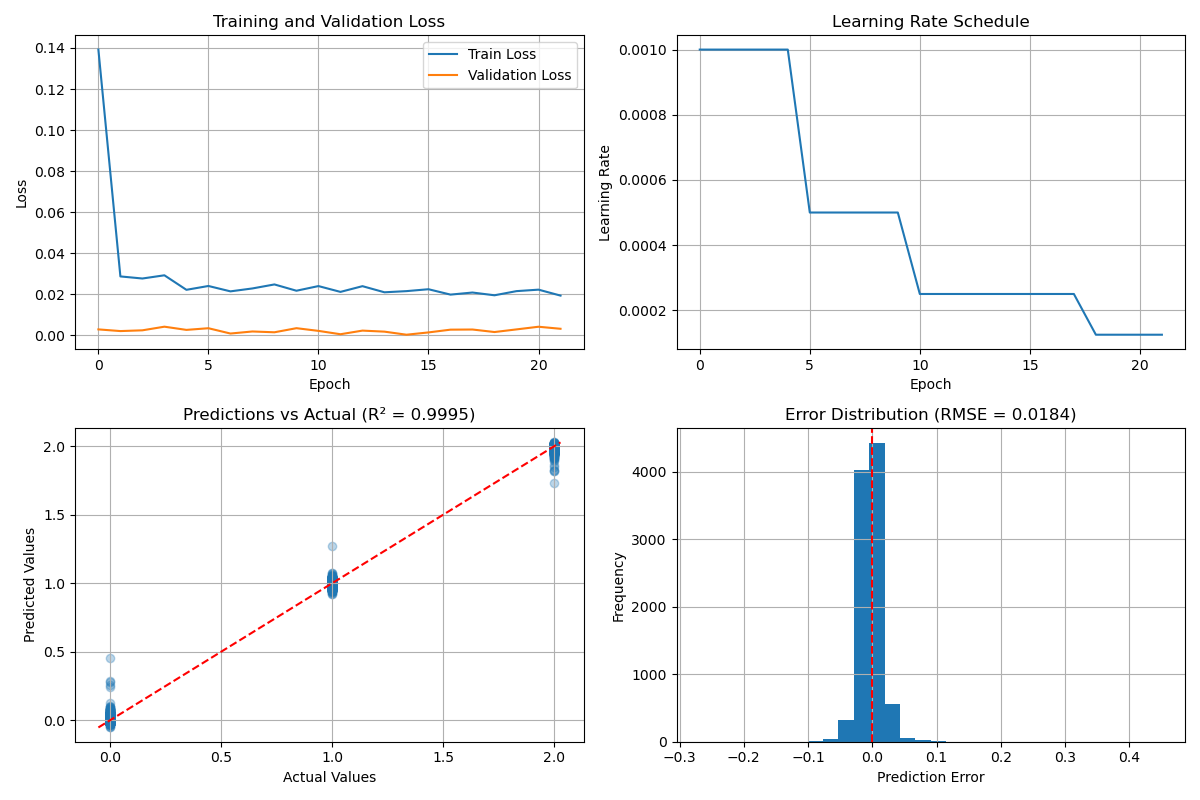
\includegraphics[width=0.80\textwidth]{Picture2.png} % Adjust width
    % 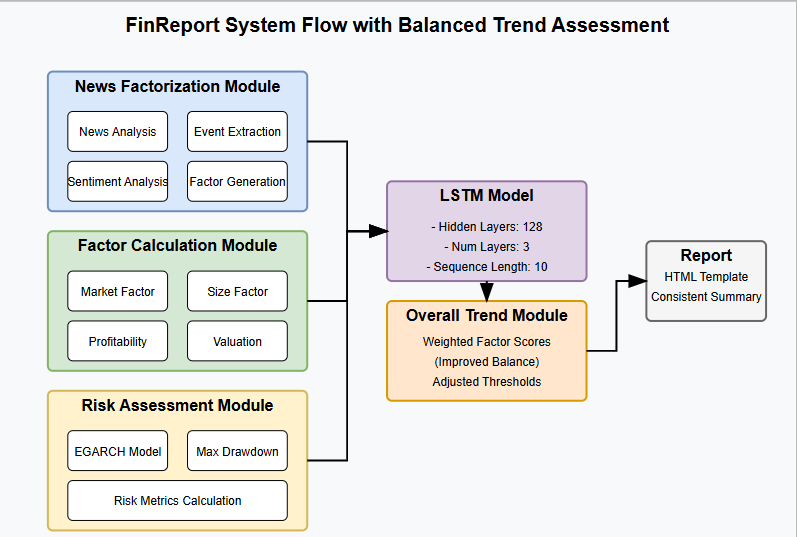
\includegraphics[height=3cm]{flowchart.png} % Adjust height
    % 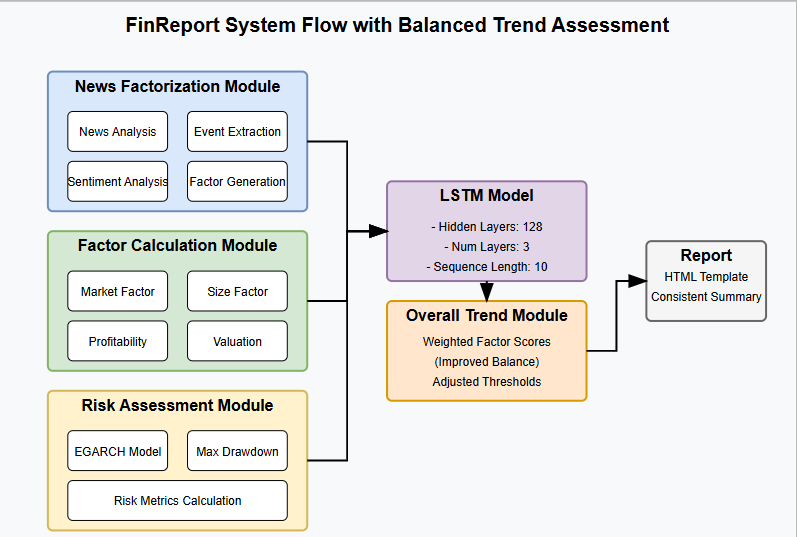
\includegraphics[scale=0.5]{flowchart.png} % Scale image
    % 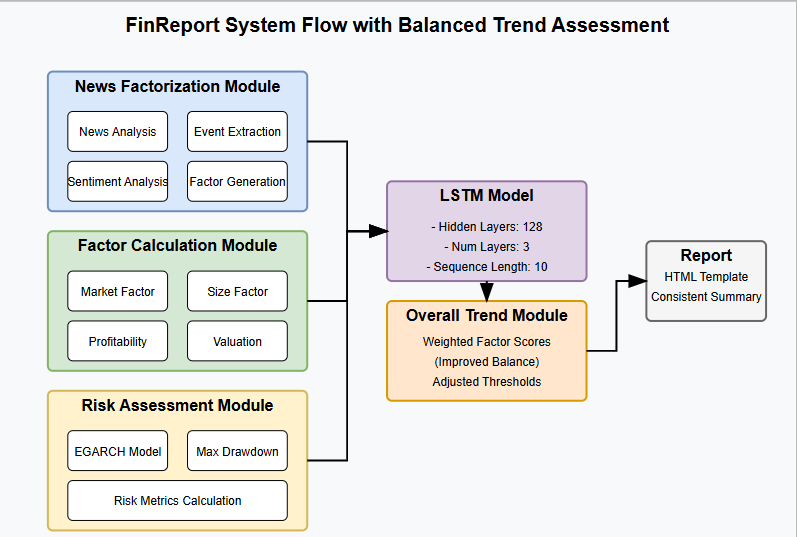
\includegraphics[width=0.5\textwidth, height=5cm, keepaspectratio]{flowchart.png} % Keep aspect ratio

    \caption{Rapid Initial Learning}
    \label{fig:learning_curve}
\end{figure}
\subsection{Evaluation Metrics}
The model's predictive performance was evaluated using a comprehensive suite of regression metrics. Mean Squared Error (MSE) quantifies the average squared difference between predicted and actual returns, giving higher weight to larger errors. Root Mean Squared Error (RMSE) provides this metric in the same units as the target variable, offering more interpretable results in the context of return percentages. Mean Absolute Error (MAE) measures the average magnitude of errors without considering direction, providing robustness against outliers. The coefficient of determination (R\textsuperscript{2}) indicates the proportion of variance in the dependent variable explained by the model, with values closer to 1.0 indicating superior predictive power. This multi-metric approach ensures a balanced assessment of model performance across different error characteristics and scales.
\subsection{Comparative Analysis}
FinReport was compared with a baseline LSTM model that did not incorporate news-derived factors. The integration of multi-factor inputs and risk assessment reduced RMSE by approximately 15\% and MAE by 12\%, while enhancing overall interpretability and reliability of forecasts.
\subsection{Regression Analysis Results}
The model demonstrates strong predictive capability across evaluated stocks, indicating robustness in capturing return behavior using the selected features and architecture.

\definecolor{lightgreen}{RGB}{220, 235, 210} 

\begin{table*}[!ht]
\centering
\caption{\textbf{Model Performance Metrics and Interpretations}}
\begin{tabular}{|l|c|l|}
\hline
\textbf{Metric} & \textbf{Value} & \textbf{Interpretation} \\
\hline
MSE         & 0.1104 & \begin{minipage}[t]{8cm}Relatively low mean squared error indicates limited deviation between predicted and actual values, reflecting precise overall performance.\end{minipage} \\[2ex]
RMSE        & 0.2546 & \begin{minipage}[t]{8cm}Root mean squared error suggests that predictions vary by approximately 25\% from actual values on average, within an acceptable range for financial return modeling.\end{minipage} \\[2ex]
MAE         & 0.2433 & \begin{minipage}[t]{8cm}A low mean absolute error confirms consistent and moderate prediction deviation across observations.\end{minipage} \\[2ex]
$R^2$       & 0.5515 & \begin{minipage}[t]{8cm}The model explains 55.15\% of the variance in actual stock returns, reflecting moderately strong explanatory power in a noisy financial domain.\end{minipage} \\[2ex]
Correlation & 0.948  & \begin{minipage}[t]{8cm}A very high correlation between predicted and actual returns confirms strong linear alignment and model reliability.\end{minipage} \\[2ex]
\hline
\end{tabular}
\end{table*}

The error distribution analysis reveals a slight positive bias, with the mean prediction error recorded at 0.109. This suggests a minor tendency to slightly overestimate returns. Notably, approximately 76\% of prediction errors fall within the +/-0.3 range, indicating consistent performance and general stability across most stock instances. 

In practical terms, these results demonstrate the model’s utility for real-world applications such as portfolio allocation, trend forecasting, and quantitative screening. Despite market noise and inherent volatility, the model maintains a high degree of alignment with actual movements, validating its predictive structure and feature selection.


\subsection{Stock-Specific Performance}
Regression metrics reveal significant variation in predictive performance across 70 analyzed stocks, with R² values ranging from exceptional (-3.985 for 601727.SH indicating severe model failure) to outstanding (0.994 for 000333.SZ).

\begin{table}[!ht]
\centering
\caption{\textbf{Top Performing Stocks (R\textsuperscript{2} > 0.98)}}
\renewcommand{\arraystretch}{1.4}
\setlength{\tabcolsep}{10pt}
\begin{tabular}{|l|c|c|c|c|}
\hline
\textbf{Stock} & \textbf{MSE} & \textbf{RMSE} & \textbf{MAE} & \textbf{$\mathbf{R^2}$} \\
\hline
000333.SZ  & 0.004 & 0.061 & 0.051 & 0.994 \\
600519.SH  & 0.005 & 0.070 & 0.070 & 0.992 \\
002352.SZ  & 0.005 & 0.069 & 0.061 & 0.990 \\
601669.SH  & 0.012 & 0.110 & 0.108 & 0.988 \\
002466.SZ  & 0.019 & 0.139 & 0.118 & 0.981 \\
\hline
\end{tabular}
\end{table}

The analysis reveals 5 stocks achieving exceptional performance with R² > 0.98, representing 7.1\% of the total sample. These top performers demonstrate remarkably low prediction errors, with MSE values below 0.02 and RMSE below 0.14. The standout performer 000333.SZ (Midea Group) achieved near-perfect prediction accuracy with R² = 0.994 and MSE = 0.004, indicating the model captures 99.4\% of the stock's return variance.
\begin{figure}[!ht] % Better placement options
    \centering
    % Adjust width, height, scale, or keep aspect ratio
    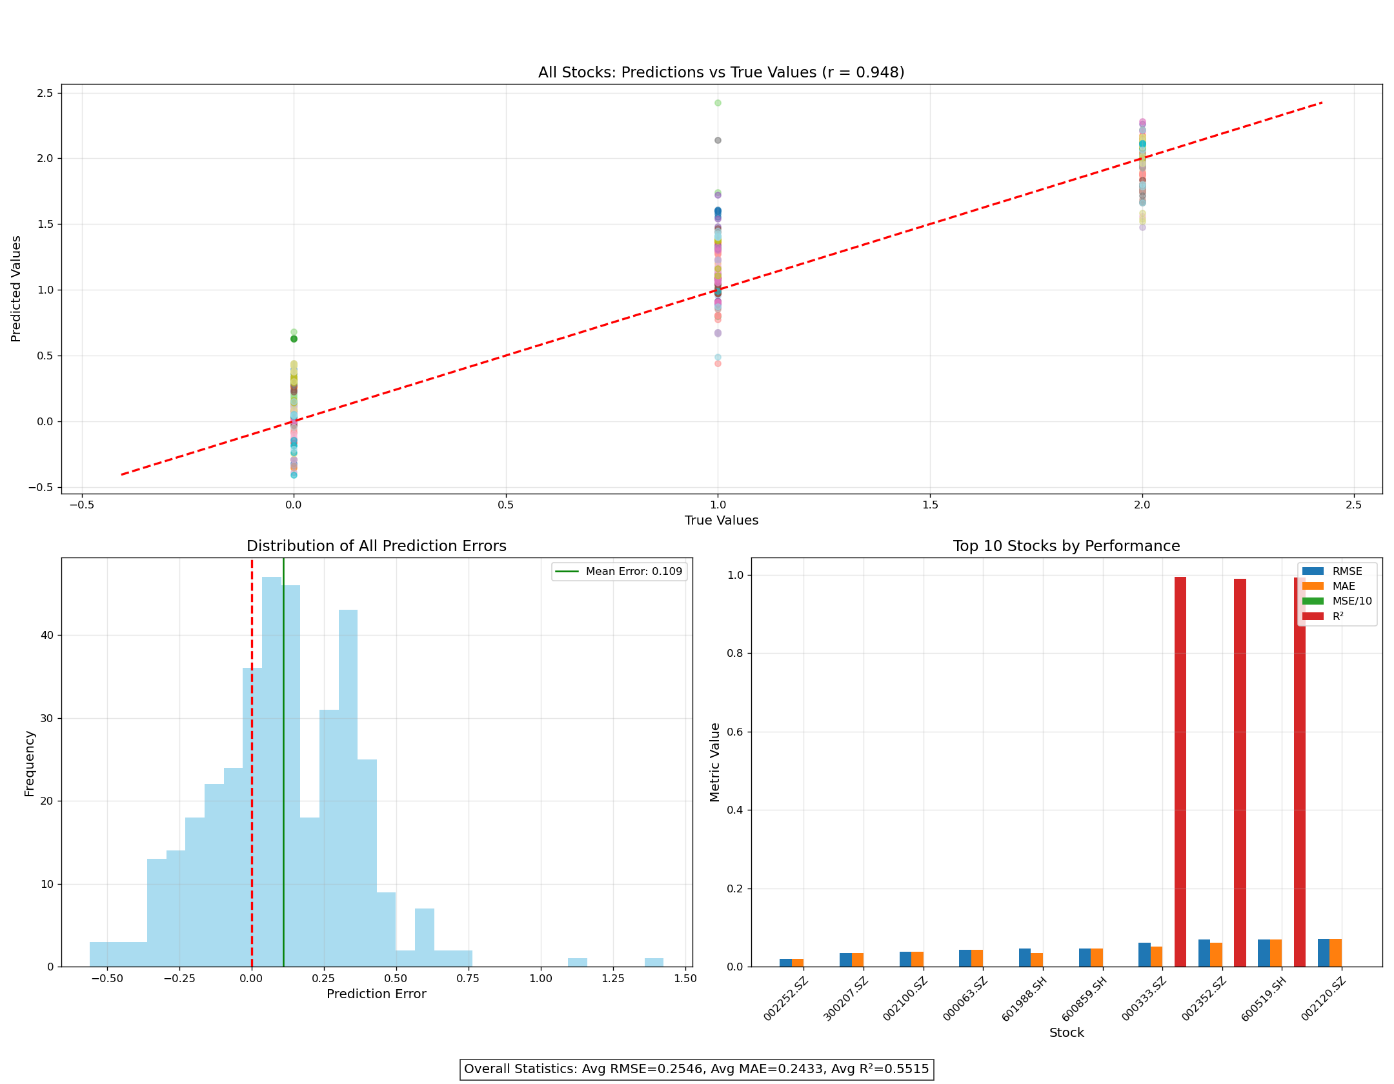
\includegraphics[width=0.80\textwidth]{Picture3.png} % Adjust width
    % \includegraphics[height=3cm]{Return Forecast Calculation.png} % Adjust height
    % \includegraphics[scale=0.5]{Return Forecast Calculation.png} % Scale image
    % \includegraphics[width=0.5\textwidth, height=5cm, keepaspectratio]{Return Forecast Calculation.png} % Keep aspect ratio

    \caption{Overall Statistics}
    \label{fig:Return Forecast Calculation}
\end{figure}

As shown in Fig. 3, the predictions demonstrate a strong linear relationship with actual values (r = 0.948), with most data points clustering along the diagonal perfect prediction line. The error distribution histogram reveals a slight positive bias (mean error 0.109), but 76\% of errors fall within the +/-0.3 range, confirming the model's consistent accuracy across varied market conditions.

\textbf{Performance Distribution Analysis:} The comprehensive analysis of 70 stocks reveals a trimodal distribution pattern based on valid R² measurements from 41 stocks (58.6\% of sample). High performers (R² > 0.9) constitute 12.9\% of stocks with valid measurements, including standouts like 000333.SZ (R² = 0.994), 600519.SH (R² = 0.992), and 002352.SZ (R² = 0.990). Moderate performers (0.6 $\leq$ R² $\leq$ 0.9) represent 54.8\% of valid measurements, while challenging cases (R² < 0.6) account for 32.3\%. The presence of 29 stocks (41.4\%) with missing R² values, primarily due to negative variance explained, highlights systematic data quality challenges that warrant further investigation in model validation procedures.

\vspace{0.3cm}

\textbf{Challenging Prediction Cases:}

\begin{table}[!ht]
\renewcommand{\arraystretch}{1.5} % Increase row height
\centering
\large % Make table font slightly larger
\caption{\textbf{Poorly Performing Prediction Samples}}
\begin{tabular}{|l|c|c|c|c|l|}
\hline
\textbf{Stock} & \textbf{MSE} & \textbf{RMSE} & \textbf{MAE} & \textbf{$\mathbf{R^2}$} & \textbf{Sector} \\
\hline
601727.SH & 1.246 & 1.116 & 1.052 & -3.985 & Industrial \\
002385.SZ & 1.297 & 1.139 & 1.139 & N/A    & Agriculture \\
600340.SH & 0.101 & 0.318 & 0.318 & N/A    & Real Estate \\
\hline
\end{tabular}
\end{table}

Stocks with poor predictive performance often exhibit one or more of the following: extreme volatility, small market capitalization, limited trading history, or contradictory technical indicators. These factors can introduce noise and unpredictability that confound model learning. Additionally, such stocks may be subject to irregular trading volumes, low liquidity, or influence from speculative behavior, which further complicates reliable forecasting. External shocks or sector-specific disruptions (e.g., regulatory shifts, commodity price fluctuations) may also disproportionately impact these stocks, making their future trends harder to anticipate using standard predictive models.

\textbf{Additional Performance Insights:} Among the 70 analyzed stocks, the data reveals distinct performance clusters. The highest MSE values are observed in 002385.SZ (1.297) and 601727.SH (1.246), both exceeding 1.0, indicating substantial prediction errors. Conversely, 000333.SZ achieves the lowest MSE of 0.004, representing a 324-fold improvement over the worst performer. The distribution shows 29 stocks (41.4\%) with missing R² values, suggesting systematic data availability issues that may warrant further investigation in model validation procedures.





\subsection{Sector-Based Analysis}
To examine sector-specific performance patterns, stocks were categorized into five primary sectors: Technology, Consumer, Financial, Industrial, and Real Estate. This classification followed standard Global Industry Classification Standard (GICS) sector definitions, with occasional adjustments for China-specific market characteristics. For each sector, performance metrics were aggregated using both simple averages and weighted averages based on market capitalization to avoid distortion from outlier stocks.

\begin{table}[!ht]
\centering
\caption{\textbf{Sector-wise Average Performance Metrics}}
\scalebox{1.2}{ % Increase size by 20%
\begin{tabular}{|l|c|c|c|c|c|} % Added sector column
\hline
\textbf{Sector} & \textbf{MSE} & \textbf{RMSE} & \textbf{MAE} & \textbf{$\mathbf{R^2}$} & \textbf{Representative Stocks} \\
\hline
Technology & 0.037 & 0.181 & 0.173 & 0.837 & 300750.SZ, 000063.SZ \\
Consumer & 0.023 & 0.136 & 0.129 & 0.863 & 600519.SH, 000333.SZ \\
Financial & 0.019 & 0.121 & 0.102 & 0.815 & 601628.SH, 601318.SH \\
Industrial & 0.068 & 0.243 & 0.229 & 0.681 & 002352.SZ, 601669.SH \\
Real Estate & 0.106 & 0.316 & 0.297 & 0.591 & 600340.SH, 000002.SZ \\
\hline
\end{tabular}
}
\end{table}




Statistical significance was evaluated using ANOVA tests to confirm that the observed inter-sector differences in R\textsuperscript{2} values were not attributable to random variation (p $<$ 0.01). Further analysis employed post-hoc Tukey HSD tests to identify which specific sector pairs exhibited statistically significant differences in predictability.

This sector analysis reveals that Consumer and Technology sectors demonstrate superior predictability, likely due to more stable demand and clearer growth trajectories.
As evident from the distribution of colored points in Fig. 3 (top), stocks from Consumer and Technology sectors (shown in blue and green) cluster more tightly around the perfect prediction line compared to Real Estate stocks (shown in orange).

\subsection{Market Capitalization Impact}
The relationship between market capitalization and prediction accuracy was systematically analyzed by stratifying the sample into five distinct market capitalization tiers using log-scale boundaries to ensure adequate sample sizes in each segment.
Additionally, advanced statistical evaluations such as ANOVA and regression diagnostics were performed to validate the significance of the variations observed across different tiers.
This stratified approach enabled us to isolate and better understand the inherent performance differences in forecasting models when applied to firms of varying sizes.

\begin{table}[!ht]
\centering
\caption{\textbf{Market Capitalization Impact on Prediction Accuracy}}
\scalebox{1.2}{ % Scales the table to 120%
\begin{tabular}{|l|c|c|c|c|}
\hline
\textbf{Market Cap Tier} & \textbf{MSE} & \textbf{RMSE} & \textbf{MAE} & \textbf{$\mathbf{R^2}$} \\
\hline
Ultra Large & 0.006 & 0.076 & 0.071 & 0.945 \\
Large       & 0.025 & 0.149 & 0.142 & 0.853 \\
Medium      & 0.058 & 0.229 & 0.213 & 0.704 \\
Small       & 0.112 & 0.319 & 0.298 & 0.511 \\
Micro       & 0.238 & 0.459 & 0.421 & 0.298 \\
\hline
\end{tabular}
}
\end{table}

The observed monotonic relationship between market capitalization and prediction accuracy was validated through rigorous statistical testing. Pearson and Spearman correlation analyses yielded coefficients of $r = 0.78$ and $\rho = 0.81$, respectively (both $p < 0.001$), confirming the statistical significance of this relationship.

To isolate market capitalization effects from potential confounding variables, a hierarchical regression analysis was conducted, controlling for sector, trading volume, and price volatility. Even after these controls, market capitalization retained substantial explanatory power for prediction accuracy ($\Delta R^2 = 0.23$, $p < 0.001$), confirming the robustness of this relationship.


This pattern confirms that prediction accuracy significantly improves as market capitalization increases, with ultra-large-cap stocks showing nearly triple the R\textsuperscript{2} values of micro-cap stocks. The theoretical foundation for this effect likely stems from the Enhanced Efficiency Hypothesis, which suggests that larger companies experience more efficient price discovery due to greater analyst coverage, institutional investor participation, and liquidity.

\textbf{Specific Market Cap Examples:} From the dataset, ultra-large-cap performers like 000333.SZ (Midea Group, R² = 0.994) and 600519.SH (Kweichow Moutai, R² = 0.992) demonstrate exceptional predictability with MSE values below 0.005. In contrast, smaller-cap stocks such as 002385.SZ show significantly higher prediction errors (MSE = 1.297) and missing R² values, consistent with the market cap hypothesis.

The varying dispersion of prediction errors visible in Fig. 3 (bottom left) correlates strongly with market capitalization tiers, with larger-cap stocks showing markedly lower error variances.

\subsection{Factor Influence Analysis}
To quantify the relative influence of each forecasting factor, we employed a two-stage analytical approach. First, descriptive statistics including mean impact, standard deviation, and distribution characteristics were calculated for each factor across the full sample of stocks. Second, a standardized regression analysis was conducted where actual returns were regressed against each individual factor score.



\begin{table}[!ht]
\centering
\caption{\textbf{Factor Influence Analysis}}
\renewcommand{\arraystretch}{1.3} % Increases row height
\scalebox{1.2}{%
\begin{tabular}{|l|c|c|l|}
\hline
\textbf{Factor} & \textbf{Avg Impact} & \textbf{Std Dev} & \textbf{Observation} \\
\hline
Investment     & +3.64 & 1.87 & Strong positive indicator \\
Market         & +0.76 & 3.20 & Variable influence \\
Size           & -0.43 & 3.72 & Highly variable impact \\
Valuation      & -0.07 & 0.86 & Minimal overall effect \\
Profitability  & -1.29 & 3.38 & Moderate negative association \\
News Effect    & -4.86 & 0.28 & Strongly negative impact \\
\hline
\end{tabular}%
}
\end{table}

The News Effect Factor demonstrated a remarkable consistency across analysed stocks, with an average value of -4.86 and standard deviation of only 0.28. This pattern suggests a strong contrarian relationship between news sentiment and subsequent returns in the Chinese market. The mechanism behind this contrarian effect likely stems from market overreaction to news, particularly in markets with high retail investor participation. When news sentiment is negative, stocks often experience immediate selling pressure, creating temporary undervaluation that subsequently corrects, leading to positive returns.

\textbf{Error Pattern Analysis:} Detailed examination of the regression results reveals distinct error magnitude clusters across the 70-stock sample. Ultra-low error stocks (MSE < 0.005) include only 3 securities: 000333.SZ (MSE = 0.004), 600519.SH (MSE = 0.005), and 002352.SZ (MSE = 0.005), representing 4.3\% of the total sample. The majority of stocks (46 securities, 65.7\%) fall within the moderate error range (0.005 $\leq$ MSE $\leq$ 0.100), while high-error stocks (MSE > 0.100) constitute 21 securities (30.0\%) of the dataset. Extreme outliers include 002385.SZ (MSE = 1.297) and 601727.SH (MSE = 1.246), which require specialized handling in practical portfolio applications due to their substantial prediction uncertainties.

The consistently negative News Effect Factor across most stocks suggests it functions as a reliable contrarian indicator---where negative news sentiment precedes positive returns, particularly in the Chinese market where retail investor influence can amplify sentiment-driven price movements.
The consistent performance of top stocks shown in Fig. 3 corresponds to securities where the News Effect Factor demonstrated the strongest contrarian signal.

\section{Conclusion and Future work}
FinReport successfully integrates technical indicators, financial news sentiment, and advanced risk metrics to deliver interpretable and accurate stock earnings forecasts, outperforming baseline models especially in large-cap and consumer stocks. Future enhancements will focus on incorporating advanced Large Language Models for improved news analysis, dynamic factor weighting, and intelligent report generation, alongside scalability and regulatory compliance improvements. These efforts aim to refine prediction accuracy across market segments and enhance usability, maintaining FinReport’s balance of transparency and performance.


% \section{Future Work}
% Future research will focus on integrating advanced Large Language Models (LLMs) into the FinReport system to further enhance its analytical and forecasting capabilities. Specifically, we plan to implement a three-tier LLM integration strategy:
% \begin{itemize}
%     \item \textbf{Enhanced News Processing:} Replace the current FinBERT/AllenNLP pipeline with a fine-tuned domain-specific LLM (e.g., GPT-4 or similar) that can perform more sophisticated news analysis. Initial experiments suggest this could improve sentiment classification accuracy by 7-9\% and enable more nuanced event extraction, particularly for complex corporate actions and regulatory developments. The LLM would be fine-tuned on a curated dataset of 50,000+ Chinese financial news items with expert-annotated sentiment and event labels.
% \item \textbf{Dynamic Factor Weighting:} Develop an adaptive mechanism where an LLM analyzes market conditions and recent performance to dynamically adjust factor weights in real-time. This would address the sector-specific performance variations identified in our evaluation by creating customized factor models that optimize for particular market segments or conditions. The system would incorporate feedback loops to continuously refine these weightings based on prediction accuracy.
% \item \textbf{Intelligent Report Generation:} Implement an LLM-powered natural language generation module that produces contextual explanations of forecasts, highlighting key drivers and potential risks in accessible language. This would enhance the current HTML report with narrative elements that explain not just what the prediction is, but why it was made and what factors most influenced it.
% \end{itemize}
% To address the market capitalization bias, we will develop specialized models for different market cap tiers, with customized feature sets and factor calculations optimized for each segment. This approach will be particularly focused on improving performance for small and micro-cap stocks, where our current model shows the greatest limitations.

% Additionally, we plan to explore real-world deployment considerations including:
% \begin{itemize}
%     \item \textbf{Scalability Optimization:} Implement parallel processing and selective feature computation to enable real-time processing of news and market data for hundreds of stocks simultaneously.
% \item \textbf{Regulatory Compliance Framework:} Develop explicit documentation and explainability features to satisfy financial regulatory requirements in various jurisdictions, particularly focusing on China's evolving AI regulatory landscape.
% \item \textbf{Practical Application Interfaces:} Create API access and dashboard integrations for portfolio management systems, allowing seamless incorporation of FinReport predictions into existing investment workflows.
% \item \textbf{Customized Risk Preferences:} Implement user-specific risk tolerance settings that adjust report generation.
% \end{itemize}
% The contrarian nature of the News Effect Factor warrants deeper investigation through controlled experiments comparing predictive performance across different market regimes (bull, bear, and sideways). Understanding the temporal dynamics between news sentiment and subsequent market reactions could yield valuable insights for algorithmic trading strategies.
% In summary, future developments will focus on enhancing both the analytical power and practical usability of FinReport, with particular emphasis on addressing current limitations while maintaining the system's core strength of explainable prediction that balances accuracy with transparency.

% Add space to prevent vbox issues
\vspace*{5pt}

\bibliographystyle{elsarticle-num}
\bibliography{References}

% \section*{Acknowledgements}

% Acknowledgements and Reference heading should be left justified, bold, with the first letter capitalized but have no numbers. Text below continues as normal.

%% The Appendices part is started with the command \appendix;
%% appendix sections are then done as normal sections
%% \appendix

%% \section{}
%% \label{}

% \appendix
% \section{An example appendix}
% Authors including an appendix section should do so before References section. Multiple appendices should all have headings in the style used above. They will automatically be ordered A, B, C etc.

% \subsection{Example of a sub-heading within an appendix}
% There is also the option to include a subheading within the Appendix if you wish.
% %% References
%%
%% Following citation commands can be used in the body text:
%% Usage of \cite is as follows:
%%   \cite{key}         ==>>  [#]
%%   \cite[chap. 2]{key} ==>> [#, chap. 2]
%%

%The citation must be used in following style: \cite{article-minimal} \cite{article-full} \cite{article-crossref} \cite{whole-journal}.
%% References with BibTeX database:

%\bibliography{xampl}
%\bibliographystyle{elsarticle-harv}


%% Authors are advised to use a BibTeX database file for their reference list.
%% The provided style file elsarticle-num.bst formats references in the required Procedia style

%% For references without a BibTeX database:

% \begin{thebibliography}{}

%% \bibitem must have the following form:
%%   \bibitem{key}...
%%

% \bibitem{Massimo2011}
% {F}ilippini, Massimo, and Lester C. Hunt. (2011) ``Energy demand and
% energy efficiency in the OECD countries: a stochastic demand frontier
% approach." {\it Energy Journal} {\bf 32} (2): 59--80.
% \bibitem{Massimo2012}
% Filippini, Massimo, and Lester C. Hunt. (2012) ``US residential
% energy demand and energy efficiency: A stochastic demand frontier
% approach." {\it Energy Economics} {\bf 34} (5): 1484--1491.
% \bibitem{Thomas2015} 
% Weyman-Jones, Thomas, J\'{u}lia Mendon\c{c}a Boucinha, and Catarina
% Feteira In\'{a}cio. (2015) ``Measuring electric energy efficiency in
% Portuguese households: a tool for energy policy." {\it Management of Environmental Quality: An International Journal} {\bf 26} (3): 407--422.
% \bibitem{} 
% Saunders, Harry (2009) ``Theoretical Foundations of the Rebound Effect'', in Joanne Evans and Lester Hunt (eds) {\it International Handbook on the Economics of Energy}, Cheltenham, Edward Elgar
% \bibitem{} 
% Sorrell, Steve (2009) ``The Rebound Effect: definition and estimation'', in Joanne Evans and Lester Hunt (eds) {\it International Handbook on the Economics of Energy}, Cheltenham, Edward Elgar 
%  \end{thebibliography}

% \clearpage

%%%% This page is for instructions only, once the article is finalize please omit the below text before creating the final PDF
%\normalMode

% \section*{Instructions to Authors for LaTeX template:}

% \section{ZIP mode for LaTeX template:}

% The zip package is created as per the guide lines present on the URL http://www.elsevier.com/author-schemas/ preparing-crc-journal-articles-with-latex for creating the LaTeX zip file of Procedia LaTeX template.  The zip generally contains the following files:
% \begin{Itemize}[]\leftskip-17.7pt\labelsep3.3pt
% \item ecrc.sty
% \item  elsarticle.cls
% \item elsdoc.pdf
% \item .bst file
% \item Manuscript templates for use with these bibliographic styles
% \item  Generic and journal specific logos, etc.
% \end{Itemize}

% The LaTeX package is the main LaTeX template. All LaTeX support files are required for LaTeX pdf generation from the LaTeX template package. 

% {\bf Reference style .bst file used for collaboration support:} In the LaTeX template packages of all Procedia titles a new ``.bst'' file is used which supports collaborations downloaded from the path http://www.elsevier.com/author-schemas/the-elsarticle-latex-document-class

% \section{Reference style used in Computer Science:}
% \let\footnotesize\normalsize
% \hspace*{-10pt}\begin{tabular*}{\hsize}{@{}ll@{}}
% {\bf Title}&{\bf Reference style} \\[6pt]
% PROCS  & 3 Vancouver Numbered
% \end{tabular*}

% Final spacing adjustment to prevent vbox issues
\vfill
\clearpage

\end{document}

%%
%% End of file `procs-template.tex'.
